%% 
%% Copyright 2019-2021 Elsevier Ltd
%% 
%% This file is part of the 'CAS Bundle'.
%% --------------------------------------
%% 
%% It may be distributed under the conditions of the LaTeX Project Public
%% License, either version 1.2 of this license or (at your option) any
%% later version.  The latest version of this license is in
%%    http://www.latex-project.org/lppl.txt
%% and version 1.2 or later is part of all distributions of LaTeX
%% version 1999/12/01 or later.
%% 
%% The list of all files belonging to the 'CAS Bundle' is
%% given in the file `manifest.txt'.
%% 
%% Template article for cas-dc documentclass for 
%% double column output.

\documentclass[fleqn]{cas-sc}

\usepackage{lipsum}
\usepackage{tikz}
\usetikzlibrary{shapes, snakes, calc}

% If the frontmatter runs over more than one page
% use the longmktitle option.

%\documentclass[a4paper,fleqn,longmktitle]{cas-dc}

%\usepackage[numbers]{natbib}
%\usepackage[authoryear]{natbib}
\usepackage[authoryear,longnamesfirst]{natbib}

%%%Author macros
\def\tsc#1{\csdef{#1}{\textsc{\lowercase{#1}}\xspace}}
\tsc{WGM}
\tsc{QE}
%%%

% Uncomment and use as if needed
%\newtheorem{theorem}{Theorem}
%\newtheorem{lemma}[theorem]{Lemma}
%\newdefinition{rmk}{Remark}
%\newproof{pf}{Proof}
%\newproof{pot}{Proof of Theorem \ref{thm}}

\begin{document}
\let\WriteBookmarks\relax
\def\floatpagepagefraction{1}
\def\textpagefraction{.001}

% Short title
\shorttitle{Ambulance Dispatch}    

% Short author
%\shortauthors{Burkman, Jin, Abuhijleh, and Sun}  
\shortauthors{First, Second, Third, Fourth}  

% Main title of the paper
\title [mode = title]{Modeling the Need for an Ambulance based on Automated Crash Reports from iPhones}  

% Title footnote mark
% eg: \tnotemark[1]
%\tnotemark[<tnote number>] 
%\tnotemark[1] 

% Title footnote 1.
% eg: \tnotetext[1]{Title footnote text}
%\tnotetext[1]{Working Title} 

% First author
%
% Options: Use if required
% eg: \author[1,3]{Author Name}[type=editor,
%       style=chinese,
%       auid=000,
%       bioid=1,
%       prefix=Sir,
%       orcid=0000-0000-0000-0000,
%       facebook=<facebook id>,
%       twitter=<twitter id>,
%       linkedin=<linkedin id>,
%       gplus=<gplus id>]

%\author[<aff no>]{<author name>}[<options>]
%\author[1,2]{J. Bradford Burkman}[]
\author[1,2]{First Author}[]
% Footnote of the first author
%\fnmark[1]
% Corresponding author indication
%\cormark[1]
% Email id of the first author
%\ead{bradburkman@gmail.com}
\ead{FirstAuthor@gmail.com}
% URL of the first author
%\ead[url]{http://www.github.com/bburkman}

% Credit authorship
% eg: \credit{Conceptualization of this study, Methodology, Software}
% Options: conceptualization; data curation; formal analysis; funding acquisition; investigation; methodology; project administration; resources; software; supervision; validation; visualization; writing – original draft; and writing – review and editing.
\credit{Conceptualization, Investigation, Writing - original draft, Visualization}


%\author[1]{Miao Jin}[]
\author[1]{Second Author}[]
\credit{Supervision, Methodology, Writing - review and editing}

%\author[1,3]{Malek Abuhijleh}[]
\author[1,3]{Third Author}[]
\credit{Investigation, Methodology}

%\author[3]{Xiaoduan Sun}[]
\author[3]{Fourth Author}[]
\credit{Data curation, Writing - review and editing}






%\affiliation[1]{organization={School of Computing and Informatics, University of Louisiana at Lafayette},
\affiliation[1]{organization={School, University},
%            addressline={301 E. Lewis St}, 
%            city={Lafayette},
%          citysep={}, % Uncomment if no comma needed between city and postcode
%            state={LA},
%            postcode={70503}, 
%            country={USA}
            }

% Address/affiliation
%\affiliation[2]{organization={Louisiana School for Math, Science, and the Arts},
\affiliation[2]{organization={Other School},
%            addressline={715 University Pkwy}, 
%            city={Natchitoches},
%          citysep={}, % Uncomment if no comma needed between city and postcode
%            state={LA},
%            postcode={71457}, 
%            country={USA}
            }

%\affiliation[3]{organization={Department of Civil Engineering, University of Louisiana at Lafayette},
\affiliation[3]{organization={Other Department, University},
%            addressline={131 Rex St}, 
%            city={Lafayette},
%          citysep={}, % Uncomment if no comma needed between city and postcode
%            state={LA},
%            postcode={70504}, 
%            country={USA}
            }




% For a title note without a number/mark
%\nonumnote{}

% Here goes the abstract
\begin{abstract}
%%%%% Abstract
% I found an abstract in TRpC June 2022 with 365 words.
%Put abstract here.
%%%%% Abstract
% I found an abstract in TRpC June 2022 with 365 words.
New Google Pixel phones can automatically notify police if the phone detects the deceleration profile of a crash.  From the data available from such an automatic notification, can we build a machine-learning model that will recommend whether police should immediately, perhaps automatically, dispatch an ambulance?  If the injuries are serious, time to medical care is critical, but few crashes result in serious injuries, and ambulances are in limited supply and expensive.  %Such a model will not be perfect, with many false positives (sending an ambulance when one is not needed) and some false negatives (not sending an ambulance when one is needed), but better than random.  How much better depends on several things that we will investigate.

The costs of the false positives and false negatives are very different.  The cost of sending an ambulance when one is not needed is measured in dollars, but the cost of not sending an ambulance when one is needed is measured in lives.  Each society chooses a marginal ethical tradeoff rate $\omega = \Delta FP/\Delta TP$ when it sets government budgets.  For our work we arbitrarily chose $\omega=2.0$ and incorporated it into the model in the class weight and decision threshold.  

We will show that the quality of the model depends mostly on what information is available to inform the decision of whether to immediately dispatch an ambulance.  
We used the data of the Crash Report Sampling System (CRSS), which is freely available online.  We have applied new methods (for this dataset in the literature) to handle missing data, and we have investigated several methods for handling the data imbalance.  To promote discussion and future research, we have included all of the code we used in our analysis.  
%\vskip 1in

\end{abstract}

% Use if graphical abstract is present
%\begin{graphicalabstract}
%\includegraphics{}
%\end{graphicalabstract}

% Research highlights
\begin{highlights}
	\item  Supports transferability and benchmarking of different approaches on a public large-scale dataset.  We have attached the code we used to perform the analysis on the Crash Report Sampling System.  
	\item Novel Application motivated by Emerging Technology:  Machine Learning Classification Models for Dispatching Ambulances based on Automated Crash Reports
	\item New Use of Dataset:  Used Crash Report Sampling System (CRSS), which has imputed missing values for some features, but not all of the ones we wanted to use.  For the first time we have seen, we used the software the CRSS authors use for multiple imputation (IVEware) to impute missing values in more features.  
	\item Perennial Machine Learning Challenge:  Imbalanced Datasets.
\end{highlights}

% Keywords
% Each keyword is seperated by \sep
\begin{keywords}
 \sep Automated crash notification \sep Ambulance dispatch \sep Emergency medical services  \sep Machine learning \sep Imbalanced Data \sep Imputation
\end{keywords}

\maketitle

% Main text

%%%%%
%
% To Do
%
%
%%%%%

%%%%% Introduction
\section{Introduction}\label{sec:Introduction}
%%%%%~\nameref{sec:Introduction}
% Introduction
\section{Introduction}
\label{intro}

%%%
\subsection{Scenario}
\label{intro_scenario}

In the (fictitious) city of Springfield, the city council and mayor are debating whether to immediately dispatch ambulances based on automated notifications from cell phones.  Many residents have cell phones (iPhones and Google Pixels) whose accelerometers will detect the deceleration profile of a crash and automatically notify the emergency call center, which immediately dispatches a police officer.  The city leaders are pleased that, because of the automated notifications, the police response to the crash scene is faster.  Should they also immediately dispatch an ambulance, making the medical response faster?

Traditionally, the emergency call center did not know about a crash until an eyewitness called, and the eyewitness could say whether the crash persons needed an ambulance, but that information does not come with an automated crash notification from a cell phone. The notification will come with a location, the emergency dispatcher already has some information (time of day, day of week, weather, urbanicity), and the cell service provider may provide some information about the primary user of the cell phone (age, sex).  With that information, the emergency dispatcher has three options.

\begin{description}
	\item [Always] immediately dispatch an ambulance, most of which will not be needed
	\item [Never] immediately dispatch an ambulance; instead, wait for a call from an eyewitness.  Many of the ambulances eventually sent to crashes had a cell phone notification and could have been sent sooner.  
	\item [Sometimes]  Develop and implement an AI recommendation system to decide which to send immediately, reserving the option to send an ambulance later based on information from an eyewitness.  
\end{description}


In Springfield today, without immediate ambulance dispatch based on automated crash notifications from cell phones, 50\% of dispatched ambulances go to automobile crashes and 10\% of crash persons need an ambulance.  Twenty percent of the crashes first have an automated notification from a cell phone before a call from an eyewitness telling whether or not the crash person needs an ambulance.  The other 80\% of crashes only have an eyewitness call.  Of the crashes with automated notifications from cell phones, 15\% will need an ambulance, 
%($\text{P} = \text{FN} + \text{TP}$), 
and 85\% will not. 
%($\text{N} = \text{TN} + \text{FP}$).  
In Figure \ref{intro_springfield_before} we have scaled the numbers per 100 ambulances sent before implementation of immediate ambulance dispatch.  

[We chose these numbers for clarity of illustration; an actual implementation would use local data.  For details on the 85/15 split, see \S\ref{dataset} Dataset and \S\ref{simplifying_assumptions} Simplifying Assumptions.]

\begin{figure}[h]
	% Image 15 cm wide
% Add 0.5cm on right for margin
\noindent\begin{tikzpicture}[x=0.02727cm, y=0.5cm, font=\normalfont\normalsize]
	\path (568,0) circle (0pt); % Add 0.5 cm on right for margin
	\draw [color=black] (0,0) -- (550,0);
	\draw [color=black] (0,2) -- (0,-1);
	\draw [color=black] (50,2) -- (50,-1);
	\draw [color=black] (100,2) -- (100,-1);
	\draw [color=black] (550,2) -- (550,-1);
	\node (A) at (25,0) {};
	\node (B) [above=-2pt of A, align=center, text=black] {
		Non-Crash \\ Needs \\ Amb \\[0.5em] 50
	};
	\node (C) at (75,0) {};
	\node (D) [above=-2pt of C, align=center, text=black] {
		Crash \\ Needs \\ Amb \\[0.5em] 50
	};
	\node (E) at (325,0) {};
	\node (F) [above=-2pt of E, align=center, text=black] {
		Crash Does Not Need Ambulance \\ No Ambulance Sent \\[0.5em]  450
	};
	\draw [color=black] (85,0) -- (85,-1);
	\draw [color=black] (185,0) -- (185,-1);
	\path (85,0) -- (100,0) node [below, midway, color=black] {
		15
		};
	\path (100,0) -- (185,0) node [below, midway, color=black] {
		85
	};
	
	\draw [<->, color=black]  (86,-2) -- (184,-2) 
		node [midway, color=black, fill=white, align=center] 
		{Automated \\ Notifications};
%	
%	\path (85,-1) -- (185,-1) node 
%		[below, midway, color=black, align=center] {
%		Automated \\ Notifications
%	};
\end{tikzpicture}

\caption{\normalfont\normalsize Springfield before implementing immediate dispatch of ambulances.  Figure accompanies \S\ref{intro_scenario}}
\label{intro_springfield_before}
\end{figure}

\FloatBarrier

If Springfield were to implement an AI recommendation system to immediately dispatch ambulances based on automated calls from cell phones, the recommendations would not perfectly predict which crash persons need an ambulance.    See Figure \ref{intro_springfield_after}, where we have zoomed in on the left side of Figure \ref{intro_springfield_before}. In our per-100-ambulances-currently-sent proportions, the recommendation system would classify each of the automated notifications as needing or not needing an ambulance.  

Of the fifteen automated crash notifications that need an ambulance, the system would correctly classify some of them as needing an ambulance (True Positive, TP), and those crash persons would get medical attention more promptly, which is the goal and benefit of the recommendation system.  The rest of those fifteen would be incorrectly classified as probably not needing an ambulance with a recommendation to wait for a call from an eyewitness before sending one (False Negative, FN).  Note that the false negatives get an ambulance just as quickly under the new system as under the old,  with an ambulance dispatched upon call from an eyewitness.  

Of the 85 automated notifications that do not need an ambulance, some would be correctly classified (True Negative, TN), but some would be incorrectly classified and we would immediately dispatch an unneeded ambulance (False Positive, FP).  Besides the cost of administration, those additional ambulance runs are the cost of immediately dispatching ambulances.  In the short term those additional ambulance runs could be more than current resources (ambulances and their teams) could handle, and in the long term could be unnacceptably expensive.  

\begin{figure}[h]
	\begin{tikzpicture}[x=0.075cm, y=0.6cm, font=\normalfont\normalsize] % 15 cm wide
	\path (207,0) circle (0pt);
	\draw [color=black] (0,0) -- (190,0);
	\draw [color=black, dashed] (190,0) -- (200,0);
	\draw [color=black] (0,2) -- (0,-1);
	\draw [color=black] (50,2) -- (50,-1);
	\draw [color=black] (100,2) -- (100,-1.5);
	\draw [color=black] (120,2) -- (120,-1);
	\node (A) at (25,0) {};
	\node (B) [above=-2pt of A, align=center, text=black] {
		Non-Crash \\ Needs Ambulance \\[0.5em] 50
	};
	\node (C) at (75,0) {};
	\node (D) [above=-2pt of C, align=center, text=black] {
		Crash \\ Needs Ambulance \\[0.5em] 50
	};
	\node (E) at (200,0) {};
	\node (F) [above left =-2pt and 0pt of E, align=right, text=black] {
		Crash Does Not Need Ambulance \\ No Ambulance Sent \\[0.5em] 450
	};
	\node (G) at (110,0) {};
	\node (H) [above=-2pt of G, align=center, text=black] {
		False \\ Alarm \\[0.5em] ?
	};

	\draw [color=black] (85,0) -- (85,-1.5);
	\draw [color=black] (185,0) -- (185,-1.5);
%	\path (85,-2) -- (100,-2) node [below, midway, color=black] {15};
%	\path (100,-1) -- (185,-1) node [below, midway, color=black] {85};
	
	\draw [<->, color=black]  (100.5,-2) -- (185,-2) 
		node [midway, color=black, fill=white, align=center] 
		{85};

	\draw [<->, color=black]  (85,-2) -- (99.5,-2) 
		node [midway, color=black, fill=white, align=center] 
		{15};

	\draw [<->, color=black]  (50,-3) -- (92,-3) 
		node [midway, color=black, fill=white, align=center] 
		{Eyewitness};

	\draw [<->, color=black]  (93,-3) -- (120,-3) 
		node [midway, color=black, fill=white, align=center] 
		{Immediate};

	\draw [<->, color=black]  (85,-4) -- (185,-4) 
		node [midway, color=black, fill=white, align=center] 
		{Automated Notifications};

	\draw [<->, color=black]  (0,3) -- (100,3) 
		node [midway, color=black, fill=white, align=center] 
		{Ambulance Needed};

	\draw [<->, color=black]  (0,4) -- (120,4) 
		node [midway, color=black, fill=white, align=center] 
		{Ambulance Sent};

%	\node (G) at (110,2) [color=black, align=left] {False \\  Alarm};
	\path (100,-0.5) -- (120,-0.5) node [midway, color=black] {FP};
	\path (120,-0.5) -- (185,-0.5) node [midway, color=black] {TN};
	\draw [color=black] (92.5,0) -- (92.5,-1.5);
	\path (85,-0.5) -- (92.5,-0.5) node [midway, color=black] {F};
	\path (85,-1.2) -- (92.5,-1.0) node [midway, color=black] {N};
	\path (100,-0.5) -- (92.5,-0.5) node [midway, color=black] {T};
	\path (100,-1.2) -- (92.5,-1.0) node [midway, color=black] {P};
\end{tikzpicture}

\caption{\normalfont\normalsize Springfield after implementing immediate dispatch of ambulances.  Figure accompanies \S\ref{intro_scenario}}
\label{intro_springfield_after}
\end{figure}

\FloatBarrier

The leaders of Springfield need to choose a balance between the benefit of more prompt medical attention and the cost of sending more ambulances.  The tradeoff of lives and money is not ethically or morally comfortable, but that is the choice governments make when they set budgets for health care and emergency services.  In the confusion matrices in Figure \ref{intro_confusion}, Springfield would love to increase TP without increasing FP, but the recommendation system will not give perfect predictions.  

\begin{figure}[h]
\begin{minipage}{\linewidth}
{\normalfont\normalsize
\begin{tabular}{p{2in}p{3in}}
\begin{tabular}{c c  | c | c | c}
	& \multicolumn{1}{c}{} & \multicolumn{2}{c}{Prediction}  \cr
	&\multicolumn{1}{c}{} & \multicolumn{1}{c}{PN} & \multicolumn{1}{c}{PP} \cr\cline{3-4}
	\multirow{2}{*}{Actual} & N & TN & FP \vrule width 0pt height 10pt depth 2pt \cr\cline{3-4}
	 & P & FN & TP	\vrule width 0pt height 10pt depth 4pt \cr\cline{3-4}
\end{tabular}
&
\begin{tabular}{c c  | c | c | c}
	\multicolumn{2}{@{}l}{Recommendation} & \multicolumn{1}{ @{} c @{} }{Wait for Call} & \multicolumn{1}{ @{} c @{} }{Immediately}   \cr
	&\multicolumn{1}{ @{} c @{} }{} & \multicolumn{1}{ @{} c @{} }{from Eyewitness} & \multicolumn{1}{ @{} c @{} }{Dispatch} \cr\cline{3-4}
	Needs & No & Correct & Increased Cost
		\vrule width 0pt height 10pt depth 2pt \cr\cline{3-4}
	Ambulance? \ \ &Yes & 
		Normal Delay & \ Prompt Medical Help \
		\vrule width 0pt height 10pt depth 4pt \cr\cline{3-4}
\end{tabular}
\cr		
\end{tabular}
}
\end{minipage}
\caption{\normalfont\normalsize Confusion matrix for ambulance dispatch.  Figure accompanies \S\ref{intro_scenario}}
\label{intro_confusion}
\end{figure}

\FloatBarrier

Building Springfield's AI recommendation system starts with an historical dataset with the features the emergency dispatchers will have at the time of the automated notification, (time of day, weather, maybe age and sex, possibly more information) and whether that historical crash person needed an ambulance (supervised learning).  A machine learning algorithm learns a model of the data, and when an automated crash notification comes in, given the data available, the model returns a value $p \in [0,1]$ that increases with the probability that the crash person needs an ambulance.  The city council and mayor need to choose a decision threshold $\theta$ such that if, for a particular crash notification, $p>\theta$, then immediately dispatch an ambulance; if $p<\theta$, wait for a call from an eyewitness.  Choosing a decision threshold of $p=1$ would mean never immediately dispatching an ambulance, and choosing $p=0$ would be always; the town leaders want to know how to choose a $p$ between the two extremes that fits their values and their budget.

The histogram in Figure \ref{intro_ideal} shows typical model output.  The model generally gives lower $p$ values to crash persons who do not need an ambulance (Neg) and higher $p$ values to crash persons who do need an ambulance (Pos), but there is significant overlap.  The most obvious feature of the histogram is the class imbalance, that there are many more Neg than Pos, in fact $85/15 \approx 6$ Neg for each Pos.  

Given a choice of decision threshold $\theta$, Springfield would immediately dispatch ambulances to all of the crashes with a $p$ value to the right of $\theta$.  The Pos (Needs ambulance) to the right of $\theta$ would get more prompt medical attention (TP), but the Neg (Does not need ambulance) to the right of $\theta$ would be wasted ambulance runs (FP) .  At $\theta = 0.8$, TP and FP are about equal, but as we consider smaller $\theta$ the number of TP increases by smaller and smaller amounts while the number of FP grows dramatically.  

\begin{figure}[h]
\centering
	%% Creator: Matplotlib, PGF backend
%%
%% To include the figure in your LaTeX document, write
%%   \input{<filename>.pgf}
%%
%% Make sure the required packages are loaded in your preamble
%%   \usepackage{pgf}
%%
%% Also ensure that all the required font packages are loaded; for instance,
%% the lmodern package is sometimes necessary when using math font.
%%   \usepackage{lmodern}
%%
%% Figures using additional raster images can only be included by \input if
%% they are in the same directory as the main LaTeX file. For loading figures
%% from other directories you can use the `import` package
%%   \usepackage{import}
%%
%% and then include the figures with
%%   \import{<path to file>}{<filename>.pgf}
%%
%% Matplotlib used the following preamble
%%   
%%   \usepackage{fontspec}
%%   \makeatletter\@ifpackageloaded{underscore}{}{\usepackage[strings]{underscore}}\makeatother
%%
\begingroup%
\makeatletter%
\begin{pgfpicture}%
\pgfpathrectangle{\pgfpointorigin}{\pgfqpoint{4.084250in}{1.703778in}}%
\pgfusepath{use as bounding box, clip}%
\begin{pgfscope}%
\pgfsetbuttcap%
\pgfsetmiterjoin%
\definecolor{currentfill}{rgb}{1.000000,1.000000,1.000000}%
\pgfsetfillcolor{currentfill}%
\pgfsetlinewidth{0.000000pt}%
\definecolor{currentstroke}{rgb}{1.000000,1.000000,1.000000}%
\pgfsetstrokecolor{currentstroke}%
\pgfsetdash{}{0pt}%
\pgfpathmoveto{\pgfqpoint{0.000000in}{0.000000in}}%
\pgfpathlineto{\pgfqpoint{4.084250in}{0.000000in}}%
\pgfpathlineto{\pgfqpoint{4.084250in}{1.703777in}}%
\pgfpathlineto{\pgfqpoint{0.000000in}{1.703777in}}%
\pgfpathlineto{\pgfqpoint{0.000000in}{0.000000in}}%
\pgfpathclose%
\pgfusepath{fill}%
\end{pgfscope}%
\begin{pgfscope}%
\pgfsetbuttcap%
\pgfsetmiterjoin%
\definecolor{currentfill}{rgb}{1.000000,1.000000,1.000000}%
\pgfsetfillcolor{currentfill}%
\pgfsetlinewidth{0.000000pt}%
\definecolor{currentstroke}{rgb}{0.000000,0.000000,0.000000}%
\pgfsetstrokecolor{currentstroke}%
\pgfsetstrokeopacity{0.000000}%
\pgfsetdash{}{0pt}%
\pgfpathmoveto{\pgfqpoint{0.546750in}{0.498777in}}%
\pgfpathlineto{\pgfqpoint{4.034250in}{0.498777in}}%
\pgfpathlineto{\pgfqpoint{4.034250in}{1.653777in}}%
\pgfpathlineto{\pgfqpoint{0.546750in}{1.653777in}}%
\pgfpathlineto{\pgfqpoint{0.546750in}{0.498777in}}%
\pgfpathclose%
\pgfusepath{fill}%
\end{pgfscope}%
\begin{pgfscope}%
\pgfpathrectangle{\pgfqpoint{0.546750in}{0.498777in}}{\pgfqpoint{3.487500in}{1.155000in}}%
\pgfusepath{clip}%
\pgfsetbuttcap%
\pgfsetmiterjoin%
\pgfsetlinewidth{1.003750pt}%
\definecolor{currentstroke}{rgb}{0.000000,0.000000,0.000000}%
\pgfsetstrokecolor{currentstroke}%
\pgfsetdash{}{0pt}%
\pgfpathmoveto{\pgfqpoint{0.641863in}{0.498777in}}%
\pgfpathlineto{\pgfqpoint{0.705273in}{0.498777in}}%
\pgfpathlineto{\pgfqpoint{0.705273in}{0.498777in}}%
\pgfpathlineto{\pgfqpoint{0.641863in}{0.498777in}}%
\pgfpathlineto{\pgfqpoint{0.641863in}{0.498777in}}%
\pgfpathclose%
\pgfusepath{stroke}%
\end{pgfscope}%
\begin{pgfscope}%
\pgfpathrectangle{\pgfqpoint{0.546750in}{0.498777in}}{\pgfqpoint{3.487500in}{1.155000in}}%
\pgfusepath{clip}%
\pgfsetbuttcap%
\pgfsetmiterjoin%
\pgfsetlinewidth{1.003750pt}%
\definecolor{currentstroke}{rgb}{0.000000,0.000000,0.000000}%
\pgfsetstrokecolor{currentstroke}%
\pgfsetdash{}{0pt}%
\pgfpathmoveto{\pgfqpoint{0.800386in}{0.498777in}}%
\pgfpathlineto{\pgfqpoint{0.863795in}{0.498777in}}%
\pgfpathlineto{\pgfqpoint{0.863795in}{0.529695in}}%
\pgfpathlineto{\pgfqpoint{0.800386in}{0.529695in}}%
\pgfpathlineto{\pgfqpoint{0.800386in}{0.498777in}}%
\pgfpathclose%
\pgfusepath{stroke}%
\end{pgfscope}%
\begin{pgfscope}%
\pgfpathrectangle{\pgfqpoint{0.546750in}{0.498777in}}{\pgfqpoint{3.487500in}{1.155000in}}%
\pgfusepath{clip}%
\pgfsetbuttcap%
\pgfsetmiterjoin%
\pgfsetlinewidth{1.003750pt}%
\definecolor{currentstroke}{rgb}{0.000000,0.000000,0.000000}%
\pgfsetstrokecolor{currentstroke}%
\pgfsetdash{}{0pt}%
\pgfpathmoveto{\pgfqpoint{0.958909in}{0.498777in}}%
\pgfpathlineto{\pgfqpoint{1.022318in}{0.498777in}}%
\pgfpathlineto{\pgfqpoint{1.022318in}{0.736639in}}%
\pgfpathlineto{\pgfqpoint{0.958909in}{0.736639in}}%
\pgfpathlineto{\pgfqpoint{0.958909in}{0.498777in}}%
\pgfpathclose%
\pgfusepath{stroke}%
\end{pgfscope}%
\begin{pgfscope}%
\pgfpathrectangle{\pgfqpoint{0.546750in}{0.498777in}}{\pgfqpoint{3.487500in}{1.155000in}}%
\pgfusepath{clip}%
\pgfsetbuttcap%
\pgfsetmiterjoin%
\pgfsetlinewidth{1.003750pt}%
\definecolor{currentstroke}{rgb}{0.000000,0.000000,0.000000}%
\pgfsetstrokecolor{currentstroke}%
\pgfsetdash{}{0pt}%
\pgfpathmoveto{\pgfqpoint{1.117432in}{0.498777in}}%
\pgfpathlineto{\pgfqpoint{1.180841in}{0.498777in}}%
\pgfpathlineto{\pgfqpoint{1.180841in}{1.084597in}}%
\pgfpathlineto{\pgfqpoint{1.117432in}{1.084597in}}%
\pgfpathlineto{\pgfqpoint{1.117432in}{0.498777in}}%
\pgfpathclose%
\pgfusepath{stroke}%
\end{pgfscope}%
\begin{pgfscope}%
\pgfpathrectangle{\pgfqpoint{0.546750in}{0.498777in}}{\pgfqpoint{3.487500in}{1.155000in}}%
\pgfusepath{clip}%
\pgfsetbuttcap%
\pgfsetmiterjoin%
\pgfsetlinewidth{1.003750pt}%
\definecolor{currentstroke}{rgb}{0.000000,0.000000,0.000000}%
\pgfsetstrokecolor{currentstroke}%
\pgfsetdash{}{0pt}%
\pgfpathmoveto{\pgfqpoint{1.275954in}{0.498777in}}%
\pgfpathlineto{\pgfqpoint{1.339363in}{0.498777in}}%
\pgfpathlineto{\pgfqpoint{1.339363in}{1.395604in}}%
\pgfpathlineto{\pgfqpoint{1.275954in}{1.395604in}}%
\pgfpathlineto{\pgfqpoint{1.275954in}{0.498777in}}%
\pgfpathclose%
\pgfusepath{stroke}%
\end{pgfscope}%
\begin{pgfscope}%
\pgfpathrectangle{\pgfqpoint{0.546750in}{0.498777in}}{\pgfqpoint{3.487500in}{1.155000in}}%
\pgfusepath{clip}%
\pgfsetbuttcap%
\pgfsetmiterjoin%
\pgfsetlinewidth{1.003750pt}%
\definecolor{currentstroke}{rgb}{0.000000,0.000000,0.000000}%
\pgfsetstrokecolor{currentstroke}%
\pgfsetdash{}{0pt}%
\pgfpathmoveto{\pgfqpoint{1.434477in}{0.498777in}}%
\pgfpathlineto{\pgfqpoint{1.497886in}{0.498777in}}%
\pgfpathlineto{\pgfqpoint{1.497886in}{1.566783in}}%
\pgfpathlineto{\pgfqpoint{1.434477in}{1.566783in}}%
\pgfpathlineto{\pgfqpoint{1.434477in}{0.498777in}}%
\pgfpathclose%
\pgfusepath{stroke}%
\end{pgfscope}%
\begin{pgfscope}%
\pgfpathrectangle{\pgfqpoint{0.546750in}{0.498777in}}{\pgfqpoint{3.487500in}{1.155000in}}%
\pgfusepath{clip}%
\pgfsetbuttcap%
\pgfsetmiterjoin%
\pgfsetlinewidth{1.003750pt}%
\definecolor{currentstroke}{rgb}{0.000000,0.000000,0.000000}%
\pgfsetstrokecolor{currentstroke}%
\pgfsetdash{}{0pt}%
\pgfpathmoveto{\pgfqpoint{1.593000in}{0.498777in}}%
\pgfpathlineto{\pgfqpoint{1.656409in}{0.498777in}}%
\pgfpathlineto{\pgfqpoint{1.656409in}{1.598777in}}%
\pgfpathlineto{\pgfqpoint{1.593000in}{1.598777in}}%
\pgfpathlineto{\pgfqpoint{1.593000in}{0.498777in}}%
\pgfpathclose%
\pgfusepath{stroke}%
\end{pgfscope}%
\begin{pgfscope}%
\pgfpathrectangle{\pgfqpoint{0.546750in}{0.498777in}}{\pgfqpoint{3.487500in}{1.155000in}}%
\pgfusepath{clip}%
\pgfsetbuttcap%
\pgfsetmiterjoin%
\pgfsetlinewidth{1.003750pt}%
\definecolor{currentstroke}{rgb}{0.000000,0.000000,0.000000}%
\pgfsetstrokecolor{currentstroke}%
\pgfsetdash{}{0pt}%
\pgfpathmoveto{\pgfqpoint{1.751523in}{0.498777in}}%
\pgfpathlineto{\pgfqpoint{1.814932in}{0.498777in}}%
\pgfpathlineto{\pgfqpoint{1.814932in}{1.545776in}}%
\pgfpathlineto{\pgfqpoint{1.751523in}{1.545776in}}%
\pgfpathlineto{\pgfqpoint{1.751523in}{0.498777in}}%
\pgfpathclose%
\pgfusepath{stroke}%
\end{pgfscope}%
\begin{pgfscope}%
\pgfpathrectangle{\pgfqpoint{0.546750in}{0.498777in}}{\pgfqpoint{3.487500in}{1.155000in}}%
\pgfusepath{clip}%
\pgfsetbuttcap%
\pgfsetmiterjoin%
\pgfsetlinewidth{1.003750pt}%
\definecolor{currentstroke}{rgb}{0.000000,0.000000,0.000000}%
\pgfsetstrokecolor{currentstroke}%
\pgfsetdash{}{0pt}%
\pgfpathmoveto{\pgfqpoint{1.910045in}{0.498777in}}%
\pgfpathlineto{\pgfqpoint{1.973454in}{0.498777in}}%
\pgfpathlineto{\pgfqpoint{1.973454in}{1.432447in}}%
\pgfpathlineto{\pgfqpoint{1.910045in}{1.432447in}}%
\pgfpathlineto{\pgfqpoint{1.910045in}{0.498777in}}%
\pgfpathclose%
\pgfusepath{stroke}%
\end{pgfscope}%
\begin{pgfscope}%
\pgfpathrectangle{\pgfqpoint{0.546750in}{0.498777in}}{\pgfqpoint{3.487500in}{1.155000in}}%
\pgfusepath{clip}%
\pgfsetbuttcap%
\pgfsetmiterjoin%
\pgfsetlinewidth{1.003750pt}%
\definecolor{currentstroke}{rgb}{0.000000,0.000000,0.000000}%
\pgfsetstrokecolor{currentstroke}%
\pgfsetdash{}{0pt}%
\pgfpathmoveto{\pgfqpoint{2.068568in}{0.498777in}}%
\pgfpathlineto{\pgfqpoint{2.131977in}{0.498777in}}%
\pgfpathlineto{\pgfqpoint{2.131977in}{1.290140in}}%
\pgfpathlineto{\pgfqpoint{2.068568in}{1.290140in}}%
\pgfpathlineto{\pgfqpoint{2.068568in}{0.498777in}}%
\pgfpathclose%
\pgfusepath{stroke}%
\end{pgfscope}%
\begin{pgfscope}%
\pgfpathrectangle{\pgfqpoint{0.546750in}{0.498777in}}{\pgfqpoint{3.487500in}{1.155000in}}%
\pgfusepath{clip}%
\pgfsetbuttcap%
\pgfsetmiterjoin%
\pgfsetlinewidth{1.003750pt}%
\definecolor{currentstroke}{rgb}{0.000000,0.000000,0.000000}%
\pgfsetstrokecolor{currentstroke}%
\pgfsetdash{}{0pt}%
\pgfpathmoveto{\pgfqpoint{2.227091in}{0.498777in}}%
\pgfpathlineto{\pgfqpoint{2.290500in}{0.498777in}}%
\pgfpathlineto{\pgfqpoint{2.290500in}{1.122624in}}%
\pgfpathlineto{\pgfqpoint{2.227091in}{1.122624in}}%
\pgfpathlineto{\pgfqpoint{2.227091in}{0.498777in}}%
\pgfpathclose%
\pgfusepath{stroke}%
\end{pgfscope}%
\begin{pgfscope}%
\pgfpathrectangle{\pgfqpoint{0.546750in}{0.498777in}}{\pgfqpoint{3.487500in}{1.155000in}}%
\pgfusepath{clip}%
\pgfsetbuttcap%
\pgfsetmiterjoin%
\pgfsetlinewidth{1.003750pt}%
\definecolor{currentstroke}{rgb}{0.000000,0.000000,0.000000}%
\pgfsetstrokecolor{currentstroke}%
\pgfsetdash{}{0pt}%
\pgfpathmoveto{\pgfqpoint{2.385613in}{0.498777in}}%
\pgfpathlineto{\pgfqpoint{2.449023in}{0.498777in}}%
\pgfpathlineto{\pgfqpoint{2.449023in}{0.989797in}}%
\pgfpathlineto{\pgfqpoint{2.385613in}{0.989797in}}%
\pgfpathlineto{\pgfqpoint{2.385613in}{0.498777in}}%
\pgfpathclose%
\pgfusepath{stroke}%
\end{pgfscope}%
\begin{pgfscope}%
\pgfpathrectangle{\pgfqpoint{0.546750in}{0.498777in}}{\pgfqpoint{3.487500in}{1.155000in}}%
\pgfusepath{clip}%
\pgfsetbuttcap%
\pgfsetmiterjoin%
\pgfsetlinewidth{1.003750pt}%
\definecolor{currentstroke}{rgb}{0.000000,0.000000,0.000000}%
\pgfsetstrokecolor{currentstroke}%
\pgfsetdash{}{0pt}%
\pgfpathmoveto{\pgfqpoint{2.544136in}{0.498777in}}%
\pgfpathlineto{\pgfqpoint{2.607545in}{0.498777in}}%
\pgfpathlineto{\pgfqpoint{2.607545in}{0.870328in}}%
\pgfpathlineto{\pgfqpoint{2.544136in}{0.870328in}}%
\pgfpathlineto{\pgfqpoint{2.544136in}{0.498777in}}%
\pgfpathclose%
\pgfusepath{stroke}%
\end{pgfscope}%
\begin{pgfscope}%
\pgfpathrectangle{\pgfqpoint{0.546750in}{0.498777in}}{\pgfqpoint{3.487500in}{1.155000in}}%
\pgfusepath{clip}%
\pgfsetbuttcap%
\pgfsetmiterjoin%
\pgfsetlinewidth{1.003750pt}%
\definecolor{currentstroke}{rgb}{0.000000,0.000000,0.000000}%
\pgfsetstrokecolor{currentstroke}%
\pgfsetdash{}{0pt}%
\pgfpathmoveto{\pgfqpoint{2.702659in}{0.498777in}}%
\pgfpathlineto{\pgfqpoint{2.766068in}{0.498777in}}%
\pgfpathlineto{\pgfqpoint{2.766068in}{0.856646in}}%
\pgfpathlineto{\pgfqpoint{2.702659in}{0.856646in}}%
\pgfpathlineto{\pgfqpoint{2.702659in}{0.498777in}}%
\pgfpathclose%
\pgfusepath{stroke}%
\end{pgfscope}%
\begin{pgfscope}%
\pgfpathrectangle{\pgfqpoint{0.546750in}{0.498777in}}{\pgfqpoint{3.487500in}{1.155000in}}%
\pgfusepath{clip}%
\pgfsetbuttcap%
\pgfsetmiterjoin%
\pgfsetlinewidth{1.003750pt}%
\definecolor{currentstroke}{rgb}{0.000000,0.000000,0.000000}%
\pgfsetstrokecolor{currentstroke}%
\pgfsetdash{}{0pt}%
\pgfpathmoveto{\pgfqpoint{2.861182in}{0.498777in}}%
\pgfpathlineto{\pgfqpoint{2.924591in}{0.498777in}}%
\pgfpathlineto{\pgfqpoint{2.924591in}{0.700766in}}%
\pgfpathlineto{\pgfqpoint{2.861182in}{0.700766in}}%
\pgfpathlineto{\pgfqpoint{2.861182in}{0.498777in}}%
\pgfpathclose%
\pgfusepath{stroke}%
\end{pgfscope}%
\begin{pgfscope}%
\pgfpathrectangle{\pgfqpoint{0.546750in}{0.498777in}}{\pgfqpoint{3.487500in}{1.155000in}}%
\pgfusepath{clip}%
\pgfsetbuttcap%
\pgfsetmiterjoin%
\pgfsetlinewidth{1.003750pt}%
\definecolor{currentstroke}{rgb}{0.000000,0.000000,0.000000}%
\pgfsetstrokecolor{currentstroke}%
\pgfsetdash{}{0pt}%
\pgfpathmoveto{\pgfqpoint{3.019704in}{0.498777in}}%
\pgfpathlineto{\pgfqpoint{3.083113in}{0.498777in}}%
\pgfpathlineto{\pgfqpoint{3.083113in}{0.650134in}}%
\pgfpathlineto{\pgfqpoint{3.019704in}{0.650134in}}%
\pgfpathlineto{\pgfqpoint{3.019704in}{0.498777in}}%
\pgfpathclose%
\pgfusepath{stroke}%
\end{pgfscope}%
\begin{pgfscope}%
\pgfpathrectangle{\pgfqpoint{0.546750in}{0.498777in}}{\pgfqpoint{3.487500in}{1.155000in}}%
\pgfusepath{clip}%
\pgfsetbuttcap%
\pgfsetmiterjoin%
\pgfsetlinewidth{1.003750pt}%
\definecolor{currentstroke}{rgb}{0.000000,0.000000,0.000000}%
\pgfsetstrokecolor{currentstroke}%
\pgfsetdash{}{0pt}%
\pgfpathmoveto{\pgfqpoint{3.178227in}{0.498777in}}%
\pgfpathlineto{\pgfqpoint{3.241636in}{0.498777in}}%
\pgfpathlineto{\pgfqpoint{3.241636in}{0.603380in}}%
\pgfpathlineto{\pgfqpoint{3.178227in}{0.603380in}}%
\pgfpathlineto{\pgfqpoint{3.178227in}{0.498777in}}%
\pgfpathclose%
\pgfusepath{stroke}%
\end{pgfscope}%
\begin{pgfscope}%
\pgfpathrectangle{\pgfqpoint{0.546750in}{0.498777in}}{\pgfqpoint{3.487500in}{1.155000in}}%
\pgfusepath{clip}%
\pgfsetbuttcap%
\pgfsetmiterjoin%
\pgfsetlinewidth{1.003750pt}%
\definecolor{currentstroke}{rgb}{0.000000,0.000000,0.000000}%
\pgfsetstrokecolor{currentstroke}%
\pgfsetdash{}{0pt}%
\pgfpathmoveto{\pgfqpoint{3.336750in}{0.498777in}}%
\pgfpathlineto{\pgfqpoint{3.400159in}{0.498777in}}%
\pgfpathlineto{\pgfqpoint{3.400159in}{0.574294in}}%
\pgfpathlineto{\pgfqpoint{3.336750in}{0.574294in}}%
\pgfpathlineto{\pgfqpoint{3.336750in}{0.498777in}}%
\pgfpathclose%
\pgfusepath{stroke}%
\end{pgfscope}%
\begin{pgfscope}%
\pgfpathrectangle{\pgfqpoint{0.546750in}{0.498777in}}{\pgfqpoint{3.487500in}{1.155000in}}%
\pgfusepath{clip}%
\pgfsetbuttcap%
\pgfsetmiterjoin%
\pgfsetlinewidth{1.003750pt}%
\definecolor{currentstroke}{rgb}{0.000000,0.000000,0.000000}%
\pgfsetstrokecolor{currentstroke}%
\pgfsetdash{}{0pt}%
\pgfpathmoveto{\pgfqpoint{3.495273in}{0.498777in}}%
\pgfpathlineto{\pgfqpoint{3.558682in}{0.498777in}}%
\pgfpathlineto{\pgfqpoint{3.558682in}{0.550486in}}%
\pgfpathlineto{\pgfqpoint{3.495273in}{0.550486in}}%
\pgfpathlineto{\pgfqpoint{3.495273in}{0.498777in}}%
\pgfpathclose%
\pgfusepath{stroke}%
\end{pgfscope}%
\begin{pgfscope}%
\pgfpathrectangle{\pgfqpoint{0.546750in}{0.498777in}}{\pgfqpoint{3.487500in}{1.155000in}}%
\pgfusepath{clip}%
\pgfsetbuttcap%
\pgfsetmiterjoin%
\pgfsetlinewidth{1.003750pt}%
\definecolor{currentstroke}{rgb}{0.000000,0.000000,0.000000}%
\pgfsetstrokecolor{currentstroke}%
\pgfsetdash{}{0pt}%
\pgfpathmoveto{\pgfqpoint{3.653795in}{0.498777in}}%
\pgfpathlineto{\pgfqpoint{3.717204in}{0.498777in}}%
\pgfpathlineto{\pgfqpoint{3.717204in}{0.534651in}}%
\pgfpathlineto{\pgfqpoint{3.653795in}{0.534651in}}%
\pgfpathlineto{\pgfqpoint{3.653795in}{0.498777in}}%
\pgfpathclose%
\pgfusepath{stroke}%
\end{pgfscope}%
\begin{pgfscope}%
\pgfpathrectangle{\pgfqpoint{0.546750in}{0.498777in}}{\pgfqpoint{3.487500in}{1.155000in}}%
\pgfusepath{clip}%
\pgfsetbuttcap%
\pgfsetmiterjoin%
\pgfsetlinewidth{1.003750pt}%
\definecolor{currentstroke}{rgb}{0.000000,0.000000,0.000000}%
\pgfsetstrokecolor{currentstroke}%
\pgfsetdash{}{0pt}%
\pgfpathmoveto{\pgfqpoint{3.812318in}{0.498777in}}%
\pgfpathlineto{\pgfqpoint{3.875727in}{0.498777in}}%
\pgfpathlineto{\pgfqpoint{3.875727in}{0.498777in}}%
\pgfpathlineto{\pgfqpoint{3.812318in}{0.498777in}}%
\pgfpathlineto{\pgfqpoint{3.812318in}{0.498777in}}%
\pgfpathclose%
\pgfusepath{stroke}%
\end{pgfscope}%
\begin{pgfscope}%
\pgfpathrectangle{\pgfqpoint{0.546750in}{0.498777in}}{\pgfqpoint{3.487500in}{1.155000in}}%
\pgfusepath{clip}%
\pgfsetbuttcap%
\pgfsetmiterjoin%
\definecolor{currentfill}{rgb}{0.000000,0.000000,0.000000}%
\pgfsetfillcolor{currentfill}%
\pgfsetlinewidth{0.000000pt}%
\definecolor{currentstroke}{rgb}{0.000000,0.000000,0.000000}%
\pgfsetstrokecolor{currentstroke}%
\pgfsetstrokeopacity{0.000000}%
\pgfsetdash{}{0pt}%
\pgfpathmoveto{\pgfqpoint{0.705273in}{0.498777in}}%
\pgfpathlineto{\pgfqpoint{0.768682in}{0.498777in}}%
\pgfpathlineto{\pgfqpoint{0.768682in}{0.498777in}}%
\pgfpathlineto{\pgfqpoint{0.705273in}{0.498777in}}%
\pgfpathlineto{\pgfqpoint{0.705273in}{0.498777in}}%
\pgfpathclose%
\pgfusepath{fill}%
\end{pgfscope}%
\begin{pgfscope}%
\pgfpathrectangle{\pgfqpoint{0.546750in}{0.498777in}}{\pgfqpoint{3.487500in}{1.155000in}}%
\pgfusepath{clip}%
\pgfsetbuttcap%
\pgfsetmiterjoin%
\definecolor{currentfill}{rgb}{0.000000,0.000000,0.000000}%
\pgfsetfillcolor{currentfill}%
\pgfsetlinewidth{0.000000pt}%
\definecolor{currentstroke}{rgb}{0.000000,0.000000,0.000000}%
\pgfsetstrokecolor{currentstroke}%
\pgfsetstrokeopacity{0.000000}%
\pgfsetdash{}{0pt}%
\pgfpathmoveto{\pgfqpoint{0.863795in}{0.498777in}}%
\pgfpathlineto{\pgfqpoint{0.927204in}{0.498777in}}%
\pgfpathlineto{\pgfqpoint{0.927204in}{0.503841in}}%
\pgfpathlineto{\pgfqpoint{0.863795in}{0.503841in}}%
\pgfpathlineto{\pgfqpoint{0.863795in}{0.498777in}}%
\pgfpathclose%
\pgfusepath{fill}%
\end{pgfscope}%
\begin{pgfscope}%
\pgfpathrectangle{\pgfqpoint{0.546750in}{0.498777in}}{\pgfqpoint{3.487500in}{1.155000in}}%
\pgfusepath{clip}%
\pgfsetbuttcap%
\pgfsetmiterjoin%
\definecolor{currentfill}{rgb}{0.000000,0.000000,0.000000}%
\pgfsetfillcolor{currentfill}%
\pgfsetlinewidth{0.000000pt}%
\definecolor{currentstroke}{rgb}{0.000000,0.000000,0.000000}%
\pgfsetstrokecolor{currentstroke}%
\pgfsetstrokeopacity{0.000000}%
\pgfsetdash{}{0pt}%
\pgfpathmoveto{\pgfqpoint{1.022318in}{0.498777in}}%
\pgfpathlineto{\pgfqpoint{1.085727in}{0.498777in}}%
\pgfpathlineto{\pgfqpoint{1.085727in}{0.505887in}}%
\pgfpathlineto{\pgfqpoint{1.022318in}{0.505887in}}%
\pgfpathlineto{\pgfqpoint{1.022318in}{0.498777in}}%
\pgfpathclose%
\pgfusepath{fill}%
\end{pgfscope}%
\begin{pgfscope}%
\pgfpathrectangle{\pgfqpoint{0.546750in}{0.498777in}}{\pgfqpoint{3.487500in}{1.155000in}}%
\pgfusepath{clip}%
\pgfsetbuttcap%
\pgfsetmiterjoin%
\definecolor{currentfill}{rgb}{0.000000,0.000000,0.000000}%
\pgfsetfillcolor{currentfill}%
\pgfsetlinewidth{0.000000pt}%
\definecolor{currentstroke}{rgb}{0.000000,0.000000,0.000000}%
\pgfsetstrokecolor{currentstroke}%
\pgfsetstrokeopacity{0.000000}%
\pgfsetdash{}{0pt}%
\pgfpathmoveto{\pgfqpoint{1.180841in}{0.498777in}}%
\pgfpathlineto{\pgfqpoint{1.244250in}{0.498777in}}%
\pgfpathlineto{\pgfqpoint{1.244250in}{0.511812in}}%
\pgfpathlineto{\pgfqpoint{1.180841in}{0.511812in}}%
\pgfpathlineto{\pgfqpoint{1.180841in}{0.498777in}}%
\pgfpathclose%
\pgfusepath{fill}%
\end{pgfscope}%
\begin{pgfscope}%
\pgfpathrectangle{\pgfqpoint{0.546750in}{0.498777in}}{\pgfqpoint{3.487500in}{1.155000in}}%
\pgfusepath{clip}%
\pgfsetbuttcap%
\pgfsetmiterjoin%
\definecolor{currentfill}{rgb}{0.000000,0.000000,0.000000}%
\pgfsetfillcolor{currentfill}%
\pgfsetlinewidth{0.000000pt}%
\definecolor{currentstroke}{rgb}{0.000000,0.000000,0.000000}%
\pgfsetstrokecolor{currentstroke}%
\pgfsetstrokeopacity{0.000000}%
\pgfsetdash{}{0pt}%
\pgfpathmoveto{\pgfqpoint{1.339363in}{0.498777in}}%
\pgfpathlineto{\pgfqpoint{1.402773in}{0.498777in}}%
\pgfpathlineto{\pgfqpoint{1.402773in}{0.511812in}}%
\pgfpathlineto{\pgfqpoint{1.339363in}{0.511812in}}%
\pgfpathlineto{\pgfqpoint{1.339363in}{0.498777in}}%
\pgfpathclose%
\pgfusepath{fill}%
\end{pgfscope}%
\begin{pgfscope}%
\pgfpathrectangle{\pgfqpoint{0.546750in}{0.498777in}}{\pgfqpoint{3.487500in}{1.155000in}}%
\pgfusepath{clip}%
\pgfsetbuttcap%
\pgfsetmiterjoin%
\definecolor{currentfill}{rgb}{0.000000,0.000000,0.000000}%
\pgfsetfillcolor{currentfill}%
\pgfsetlinewidth{0.000000pt}%
\definecolor{currentstroke}{rgb}{0.000000,0.000000,0.000000}%
\pgfsetstrokecolor{currentstroke}%
\pgfsetstrokeopacity{0.000000}%
\pgfsetdash{}{0pt}%
\pgfpathmoveto{\pgfqpoint{1.497886in}{0.498777in}}%
\pgfpathlineto{\pgfqpoint{1.561295in}{0.498777in}}%
\pgfpathlineto{\pgfqpoint{1.561295in}{0.520323in}}%
\pgfpathlineto{\pgfqpoint{1.497886in}{0.520323in}}%
\pgfpathlineto{\pgfqpoint{1.497886in}{0.498777in}}%
\pgfpathclose%
\pgfusepath{fill}%
\end{pgfscope}%
\begin{pgfscope}%
\pgfpathrectangle{\pgfqpoint{0.546750in}{0.498777in}}{\pgfqpoint{3.487500in}{1.155000in}}%
\pgfusepath{clip}%
\pgfsetbuttcap%
\pgfsetmiterjoin%
\definecolor{currentfill}{rgb}{0.000000,0.000000,0.000000}%
\pgfsetfillcolor{currentfill}%
\pgfsetlinewidth{0.000000pt}%
\definecolor{currentstroke}{rgb}{0.000000,0.000000,0.000000}%
\pgfsetstrokecolor{currentstroke}%
\pgfsetstrokeopacity{0.000000}%
\pgfsetdash{}{0pt}%
\pgfpathmoveto{\pgfqpoint{1.656409in}{0.498777in}}%
\pgfpathlineto{\pgfqpoint{1.719818in}{0.498777in}}%
\pgfpathlineto{\pgfqpoint{1.719818in}{0.525494in}}%
\pgfpathlineto{\pgfqpoint{1.656409in}{0.525494in}}%
\pgfpathlineto{\pgfqpoint{1.656409in}{0.498777in}}%
\pgfpathclose%
\pgfusepath{fill}%
\end{pgfscope}%
\begin{pgfscope}%
\pgfpathrectangle{\pgfqpoint{0.546750in}{0.498777in}}{\pgfqpoint{3.487500in}{1.155000in}}%
\pgfusepath{clip}%
\pgfsetbuttcap%
\pgfsetmiterjoin%
\definecolor{currentfill}{rgb}{0.000000,0.000000,0.000000}%
\pgfsetfillcolor{currentfill}%
\pgfsetlinewidth{0.000000pt}%
\definecolor{currentstroke}{rgb}{0.000000,0.000000,0.000000}%
\pgfsetstrokecolor{currentstroke}%
\pgfsetstrokeopacity{0.000000}%
\pgfsetdash{}{0pt}%
\pgfpathmoveto{\pgfqpoint{1.814932in}{0.498777in}}%
\pgfpathlineto{\pgfqpoint{1.878341in}{0.498777in}}%
\pgfpathlineto{\pgfqpoint{1.878341in}{0.535620in}}%
\pgfpathlineto{\pgfqpoint{1.814932in}{0.535620in}}%
\pgfpathlineto{\pgfqpoint{1.814932in}{0.498777in}}%
\pgfpathclose%
\pgfusepath{fill}%
\end{pgfscope}%
\begin{pgfscope}%
\pgfpathrectangle{\pgfqpoint{0.546750in}{0.498777in}}{\pgfqpoint{3.487500in}{1.155000in}}%
\pgfusepath{clip}%
\pgfsetbuttcap%
\pgfsetmiterjoin%
\definecolor{currentfill}{rgb}{0.000000,0.000000,0.000000}%
\pgfsetfillcolor{currentfill}%
\pgfsetlinewidth{0.000000pt}%
\definecolor{currentstroke}{rgb}{0.000000,0.000000,0.000000}%
\pgfsetstrokecolor{currentstroke}%
\pgfsetstrokeopacity{0.000000}%
\pgfsetdash{}{0pt}%
\pgfpathmoveto{\pgfqpoint{1.973454in}{0.498777in}}%
\pgfpathlineto{\pgfqpoint{2.036863in}{0.498777in}}%
\pgfpathlineto{\pgfqpoint{2.036863in}{0.556304in}}%
\pgfpathlineto{\pgfqpoint{1.973454in}{0.556304in}}%
\pgfpathlineto{\pgfqpoint{1.973454in}{0.498777in}}%
\pgfpathclose%
\pgfusepath{fill}%
\end{pgfscope}%
\begin{pgfscope}%
\pgfpathrectangle{\pgfqpoint{0.546750in}{0.498777in}}{\pgfqpoint{3.487500in}{1.155000in}}%
\pgfusepath{clip}%
\pgfsetbuttcap%
\pgfsetmiterjoin%
\definecolor{currentfill}{rgb}{0.000000,0.000000,0.000000}%
\pgfsetfillcolor{currentfill}%
\pgfsetlinewidth{0.000000pt}%
\definecolor{currentstroke}{rgb}{0.000000,0.000000,0.000000}%
\pgfsetstrokecolor{currentstroke}%
\pgfsetstrokeopacity{0.000000}%
\pgfsetdash{}{0pt}%
\pgfpathmoveto{\pgfqpoint{2.131977in}{0.498777in}}%
\pgfpathlineto{\pgfqpoint{2.195386in}{0.498777in}}%
\pgfpathlineto{\pgfqpoint{2.195386in}{0.565891in}}%
\pgfpathlineto{\pgfqpoint{2.131977in}{0.565891in}}%
\pgfpathlineto{\pgfqpoint{2.131977in}{0.498777in}}%
\pgfpathclose%
\pgfusepath{fill}%
\end{pgfscope}%
\begin{pgfscope}%
\pgfpathrectangle{\pgfqpoint{0.546750in}{0.498777in}}{\pgfqpoint{3.487500in}{1.155000in}}%
\pgfusepath{clip}%
\pgfsetbuttcap%
\pgfsetmiterjoin%
\definecolor{currentfill}{rgb}{0.000000,0.000000,0.000000}%
\pgfsetfillcolor{currentfill}%
\pgfsetlinewidth{0.000000pt}%
\definecolor{currentstroke}{rgb}{0.000000,0.000000,0.000000}%
\pgfsetstrokecolor{currentstroke}%
\pgfsetstrokeopacity{0.000000}%
\pgfsetdash{}{0pt}%
\pgfpathmoveto{\pgfqpoint{2.290500in}{0.498777in}}%
\pgfpathlineto{\pgfqpoint{2.353909in}{0.498777in}}%
\pgfpathlineto{\pgfqpoint{2.353909in}{0.595085in}}%
\pgfpathlineto{\pgfqpoint{2.290500in}{0.595085in}}%
\pgfpathlineto{\pgfqpoint{2.290500in}{0.498777in}}%
\pgfpathclose%
\pgfusepath{fill}%
\end{pgfscope}%
\begin{pgfscope}%
\pgfpathrectangle{\pgfqpoint{0.546750in}{0.498777in}}{\pgfqpoint{3.487500in}{1.155000in}}%
\pgfusepath{clip}%
\pgfsetbuttcap%
\pgfsetmiterjoin%
\definecolor{currentfill}{rgb}{0.000000,0.000000,0.000000}%
\pgfsetfillcolor{currentfill}%
\pgfsetlinewidth{0.000000pt}%
\definecolor{currentstroke}{rgb}{0.000000,0.000000,0.000000}%
\pgfsetstrokecolor{currentstroke}%
\pgfsetstrokeopacity{0.000000}%
\pgfsetdash{}{0pt}%
\pgfpathmoveto{\pgfqpoint{2.449023in}{0.498777in}}%
\pgfpathlineto{\pgfqpoint{2.512432in}{0.498777in}}%
\pgfpathlineto{\pgfqpoint{2.512432in}{0.611029in}}%
\pgfpathlineto{\pgfqpoint{2.449023in}{0.611029in}}%
\pgfpathlineto{\pgfqpoint{2.449023in}{0.498777in}}%
\pgfpathclose%
\pgfusepath{fill}%
\end{pgfscope}%
\begin{pgfscope}%
\pgfpathrectangle{\pgfqpoint{0.546750in}{0.498777in}}{\pgfqpoint{3.487500in}{1.155000in}}%
\pgfusepath{clip}%
\pgfsetbuttcap%
\pgfsetmiterjoin%
\definecolor{currentfill}{rgb}{0.000000,0.000000,0.000000}%
\pgfsetfillcolor{currentfill}%
\pgfsetlinewidth{0.000000pt}%
\definecolor{currentstroke}{rgb}{0.000000,0.000000,0.000000}%
\pgfsetstrokecolor{currentstroke}%
\pgfsetstrokeopacity{0.000000}%
\pgfsetdash{}{0pt}%
\pgfpathmoveto{\pgfqpoint{2.607545in}{0.498777in}}%
\pgfpathlineto{\pgfqpoint{2.670954in}{0.498777in}}%
\pgfpathlineto{\pgfqpoint{2.670954in}{0.629773in}}%
\pgfpathlineto{\pgfqpoint{2.607545in}{0.629773in}}%
\pgfpathlineto{\pgfqpoint{2.607545in}{0.498777in}}%
\pgfpathclose%
\pgfusepath{fill}%
\end{pgfscope}%
\begin{pgfscope}%
\pgfpathrectangle{\pgfqpoint{0.546750in}{0.498777in}}{\pgfqpoint{3.487500in}{1.155000in}}%
\pgfusepath{clip}%
\pgfsetbuttcap%
\pgfsetmiterjoin%
\definecolor{currentfill}{rgb}{0.000000,0.000000,0.000000}%
\pgfsetfillcolor{currentfill}%
\pgfsetlinewidth{0.000000pt}%
\definecolor{currentstroke}{rgb}{0.000000,0.000000,0.000000}%
\pgfsetstrokecolor{currentstroke}%
\pgfsetstrokeopacity{0.000000}%
\pgfsetdash{}{0pt}%
\pgfpathmoveto{\pgfqpoint{2.766068in}{0.498777in}}%
\pgfpathlineto{\pgfqpoint{2.829477in}{0.498777in}}%
\pgfpathlineto{\pgfqpoint{2.829477in}{0.659937in}}%
\pgfpathlineto{\pgfqpoint{2.766068in}{0.659937in}}%
\pgfpathlineto{\pgfqpoint{2.766068in}{0.498777in}}%
\pgfpathclose%
\pgfusepath{fill}%
\end{pgfscope}%
\begin{pgfscope}%
\pgfpathrectangle{\pgfqpoint{0.546750in}{0.498777in}}{\pgfqpoint{3.487500in}{1.155000in}}%
\pgfusepath{clip}%
\pgfsetbuttcap%
\pgfsetmiterjoin%
\definecolor{currentfill}{rgb}{0.000000,0.000000,0.000000}%
\pgfsetfillcolor{currentfill}%
\pgfsetlinewidth{0.000000pt}%
\definecolor{currentstroke}{rgb}{0.000000,0.000000,0.000000}%
\pgfsetstrokecolor{currentstroke}%
\pgfsetstrokeopacity{0.000000}%
\pgfsetdash{}{0pt}%
\pgfpathmoveto{\pgfqpoint{2.924591in}{0.498777in}}%
\pgfpathlineto{\pgfqpoint{2.988000in}{0.498777in}}%
\pgfpathlineto{\pgfqpoint{2.988000in}{0.684822in}}%
\pgfpathlineto{\pgfqpoint{2.924591in}{0.684822in}}%
\pgfpathlineto{\pgfqpoint{2.924591in}{0.498777in}}%
\pgfpathclose%
\pgfusepath{fill}%
\end{pgfscope}%
\begin{pgfscope}%
\pgfpathrectangle{\pgfqpoint{0.546750in}{0.498777in}}{\pgfqpoint{3.487500in}{1.155000in}}%
\pgfusepath{clip}%
\pgfsetbuttcap%
\pgfsetmiterjoin%
\definecolor{currentfill}{rgb}{0.000000,0.000000,0.000000}%
\pgfsetfillcolor{currentfill}%
\pgfsetlinewidth{0.000000pt}%
\definecolor{currentstroke}{rgb}{0.000000,0.000000,0.000000}%
\pgfsetstrokecolor{currentstroke}%
\pgfsetstrokeopacity{0.000000}%
\pgfsetdash{}{0pt}%
\pgfpathmoveto{\pgfqpoint{3.083113in}{0.498777in}}%
\pgfpathlineto{\pgfqpoint{3.146523in}{0.498777in}}%
\pgfpathlineto{\pgfqpoint{3.146523in}{0.698934in}}%
\pgfpathlineto{\pgfqpoint{3.083113in}{0.698934in}}%
\pgfpathlineto{\pgfqpoint{3.083113in}{0.498777in}}%
\pgfpathclose%
\pgfusepath{fill}%
\end{pgfscope}%
\begin{pgfscope}%
\pgfpathrectangle{\pgfqpoint{0.546750in}{0.498777in}}{\pgfqpoint{3.487500in}{1.155000in}}%
\pgfusepath{clip}%
\pgfsetbuttcap%
\pgfsetmiterjoin%
\definecolor{currentfill}{rgb}{0.000000,0.000000,0.000000}%
\pgfsetfillcolor{currentfill}%
\pgfsetlinewidth{0.000000pt}%
\definecolor{currentstroke}{rgb}{0.000000,0.000000,0.000000}%
\pgfsetstrokecolor{currentstroke}%
\pgfsetstrokeopacity{0.000000}%
\pgfsetdash{}{0pt}%
\pgfpathmoveto{\pgfqpoint{3.241636in}{0.498777in}}%
\pgfpathlineto{\pgfqpoint{3.305045in}{0.498777in}}%
\pgfpathlineto{\pgfqpoint{3.305045in}{0.682129in}}%
\pgfpathlineto{\pgfqpoint{3.241636in}{0.682129in}}%
\pgfpathlineto{\pgfqpoint{3.241636in}{0.498777in}}%
\pgfpathclose%
\pgfusepath{fill}%
\end{pgfscope}%
\begin{pgfscope}%
\pgfpathrectangle{\pgfqpoint{0.546750in}{0.498777in}}{\pgfqpoint{3.487500in}{1.155000in}}%
\pgfusepath{clip}%
\pgfsetbuttcap%
\pgfsetmiterjoin%
\definecolor{currentfill}{rgb}{0.000000,0.000000,0.000000}%
\pgfsetfillcolor{currentfill}%
\pgfsetlinewidth{0.000000pt}%
\definecolor{currentstroke}{rgb}{0.000000,0.000000,0.000000}%
\pgfsetstrokecolor{currentstroke}%
\pgfsetstrokeopacity{0.000000}%
\pgfsetdash{}{0pt}%
\pgfpathmoveto{\pgfqpoint{3.400159in}{0.498777in}}%
\pgfpathlineto{\pgfqpoint{3.463568in}{0.498777in}}%
\pgfpathlineto{\pgfqpoint{3.463568in}{0.647118in}}%
\pgfpathlineto{\pgfqpoint{3.400159in}{0.647118in}}%
\pgfpathlineto{\pgfqpoint{3.400159in}{0.498777in}}%
\pgfpathclose%
\pgfusepath{fill}%
\end{pgfscope}%
\begin{pgfscope}%
\pgfpathrectangle{\pgfqpoint{0.546750in}{0.498777in}}{\pgfqpoint{3.487500in}{1.155000in}}%
\pgfusepath{clip}%
\pgfsetbuttcap%
\pgfsetmiterjoin%
\definecolor{currentfill}{rgb}{0.000000,0.000000,0.000000}%
\pgfsetfillcolor{currentfill}%
\pgfsetlinewidth{0.000000pt}%
\definecolor{currentstroke}{rgb}{0.000000,0.000000,0.000000}%
\pgfsetstrokecolor{currentstroke}%
\pgfsetstrokeopacity{0.000000}%
\pgfsetdash{}{0pt}%
\pgfpathmoveto{\pgfqpoint{3.558682in}{0.498777in}}%
\pgfpathlineto{\pgfqpoint{3.622091in}{0.498777in}}%
\pgfpathlineto{\pgfqpoint{3.622091in}{0.599071in}}%
\pgfpathlineto{\pgfqpoint{3.558682in}{0.599071in}}%
\pgfpathlineto{\pgfqpoint{3.558682in}{0.498777in}}%
\pgfpathclose%
\pgfusepath{fill}%
\end{pgfscope}%
\begin{pgfscope}%
\pgfpathrectangle{\pgfqpoint{0.546750in}{0.498777in}}{\pgfqpoint{3.487500in}{1.155000in}}%
\pgfusepath{clip}%
\pgfsetbuttcap%
\pgfsetmiterjoin%
\definecolor{currentfill}{rgb}{0.000000,0.000000,0.000000}%
\pgfsetfillcolor{currentfill}%
\pgfsetlinewidth{0.000000pt}%
\definecolor{currentstroke}{rgb}{0.000000,0.000000,0.000000}%
\pgfsetstrokecolor{currentstroke}%
\pgfsetstrokeopacity{0.000000}%
\pgfsetdash{}{0pt}%
\pgfpathmoveto{\pgfqpoint{3.717204in}{0.498777in}}%
\pgfpathlineto{\pgfqpoint{3.780613in}{0.498777in}}%
\pgfpathlineto{\pgfqpoint{3.780613in}{0.542622in}}%
\pgfpathlineto{\pgfqpoint{3.717204in}{0.542622in}}%
\pgfpathlineto{\pgfqpoint{3.717204in}{0.498777in}}%
\pgfpathclose%
\pgfusepath{fill}%
\end{pgfscope}%
\begin{pgfscope}%
\pgfpathrectangle{\pgfqpoint{0.546750in}{0.498777in}}{\pgfqpoint{3.487500in}{1.155000in}}%
\pgfusepath{clip}%
\pgfsetbuttcap%
\pgfsetmiterjoin%
\definecolor{currentfill}{rgb}{0.000000,0.000000,0.000000}%
\pgfsetfillcolor{currentfill}%
\pgfsetlinewidth{0.000000pt}%
\definecolor{currentstroke}{rgb}{0.000000,0.000000,0.000000}%
\pgfsetstrokecolor{currentstroke}%
\pgfsetstrokeopacity{0.000000}%
\pgfsetdash{}{0pt}%
\pgfpathmoveto{\pgfqpoint{3.875727in}{0.498777in}}%
\pgfpathlineto{\pgfqpoint{3.939136in}{0.498777in}}%
\pgfpathlineto{\pgfqpoint{3.939136in}{0.503948in}}%
\pgfpathlineto{\pgfqpoint{3.875727in}{0.503948in}}%
\pgfpathlineto{\pgfqpoint{3.875727in}{0.498777in}}%
\pgfpathclose%
\pgfusepath{fill}%
\end{pgfscope}%
\begin{pgfscope}%
\pgfsetbuttcap%
\pgfsetroundjoin%
\definecolor{currentfill}{rgb}{0.000000,0.000000,0.000000}%
\pgfsetfillcolor{currentfill}%
\pgfsetlinewidth{0.803000pt}%
\definecolor{currentstroke}{rgb}{0.000000,0.000000,0.000000}%
\pgfsetstrokecolor{currentstroke}%
\pgfsetdash{}{0pt}%
\pgfsys@defobject{currentmarker}{\pgfqpoint{0.000000in}{-0.048611in}}{\pgfqpoint{0.000000in}{0.000000in}}{%
\pgfpathmoveto{\pgfqpoint{0.000000in}{0.000000in}}%
\pgfpathlineto{\pgfqpoint{0.000000in}{-0.048611in}}%
\pgfusepath{stroke,fill}%
}%
\begin{pgfscope}%
\pgfsys@transformshift{0.546750in}{0.498777in}%
\pgfsys@useobject{currentmarker}{}%
\end{pgfscope}%
\end{pgfscope}%
\begin{pgfscope}%
\pgfsetbuttcap%
\pgfsetroundjoin%
\definecolor{currentfill}{rgb}{0.000000,0.000000,0.000000}%
\pgfsetfillcolor{currentfill}%
\pgfsetlinewidth{0.803000pt}%
\definecolor{currentstroke}{rgb}{0.000000,0.000000,0.000000}%
\pgfsetstrokecolor{currentstroke}%
\pgfsetdash{}{0pt}%
\pgfsys@defobject{currentmarker}{\pgfqpoint{0.000000in}{-0.048611in}}{\pgfqpoint{0.000000in}{0.000000in}}{%
\pgfpathmoveto{\pgfqpoint{0.000000in}{0.000000in}}%
\pgfpathlineto{\pgfqpoint{0.000000in}{-0.048611in}}%
\pgfusepath{stroke,fill}%
}%
\begin{pgfscope}%
\pgfsys@transformshift{0.705273in}{0.498777in}%
\pgfsys@useobject{currentmarker}{}%
\end{pgfscope}%
\end{pgfscope}%
\begin{pgfscope}%
\definecolor{textcolor}{rgb}{0.000000,0.000000,0.000000}%
\pgfsetstrokecolor{textcolor}%
\pgfsetfillcolor{textcolor}%
\pgftext[x=0.705273in,y=0.401555in,,top]{\color{textcolor}\rmfamily\fontsize{12.000000}{14.400000}\selectfont 0.0}%
\end{pgfscope}%
\begin{pgfscope}%
\pgfsetbuttcap%
\pgfsetroundjoin%
\definecolor{currentfill}{rgb}{0.000000,0.000000,0.000000}%
\pgfsetfillcolor{currentfill}%
\pgfsetlinewidth{0.803000pt}%
\definecolor{currentstroke}{rgb}{0.000000,0.000000,0.000000}%
\pgfsetstrokecolor{currentstroke}%
\pgfsetdash{}{0pt}%
\pgfsys@defobject{currentmarker}{\pgfqpoint{0.000000in}{-0.048611in}}{\pgfqpoint{0.000000in}{0.000000in}}{%
\pgfpathmoveto{\pgfqpoint{0.000000in}{0.000000in}}%
\pgfpathlineto{\pgfqpoint{0.000000in}{-0.048611in}}%
\pgfusepath{stroke,fill}%
}%
\begin{pgfscope}%
\pgfsys@transformshift{0.863795in}{0.498777in}%
\pgfsys@useobject{currentmarker}{}%
\end{pgfscope}%
\end{pgfscope}%
\begin{pgfscope}%
\pgfsetbuttcap%
\pgfsetroundjoin%
\definecolor{currentfill}{rgb}{0.000000,0.000000,0.000000}%
\pgfsetfillcolor{currentfill}%
\pgfsetlinewidth{0.803000pt}%
\definecolor{currentstroke}{rgb}{0.000000,0.000000,0.000000}%
\pgfsetstrokecolor{currentstroke}%
\pgfsetdash{}{0pt}%
\pgfsys@defobject{currentmarker}{\pgfqpoint{0.000000in}{-0.048611in}}{\pgfqpoint{0.000000in}{0.000000in}}{%
\pgfpathmoveto{\pgfqpoint{0.000000in}{0.000000in}}%
\pgfpathlineto{\pgfqpoint{0.000000in}{-0.048611in}}%
\pgfusepath{stroke,fill}%
}%
\begin{pgfscope}%
\pgfsys@transformshift{1.022318in}{0.498777in}%
\pgfsys@useobject{currentmarker}{}%
\end{pgfscope}%
\end{pgfscope}%
\begin{pgfscope}%
\definecolor{textcolor}{rgb}{0.000000,0.000000,0.000000}%
\pgfsetstrokecolor{textcolor}%
\pgfsetfillcolor{textcolor}%
\pgftext[x=1.022318in,y=0.401555in,,top]{\color{textcolor}\rmfamily\fontsize{12.000000}{14.400000}\selectfont 0.1}%
\end{pgfscope}%
\begin{pgfscope}%
\pgfsetbuttcap%
\pgfsetroundjoin%
\definecolor{currentfill}{rgb}{0.000000,0.000000,0.000000}%
\pgfsetfillcolor{currentfill}%
\pgfsetlinewidth{0.803000pt}%
\definecolor{currentstroke}{rgb}{0.000000,0.000000,0.000000}%
\pgfsetstrokecolor{currentstroke}%
\pgfsetdash{}{0pt}%
\pgfsys@defobject{currentmarker}{\pgfqpoint{0.000000in}{-0.048611in}}{\pgfqpoint{0.000000in}{0.000000in}}{%
\pgfpathmoveto{\pgfqpoint{0.000000in}{0.000000in}}%
\pgfpathlineto{\pgfqpoint{0.000000in}{-0.048611in}}%
\pgfusepath{stroke,fill}%
}%
\begin{pgfscope}%
\pgfsys@transformshift{1.180841in}{0.498777in}%
\pgfsys@useobject{currentmarker}{}%
\end{pgfscope}%
\end{pgfscope}%
\begin{pgfscope}%
\pgfsetbuttcap%
\pgfsetroundjoin%
\definecolor{currentfill}{rgb}{0.000000,0.000000,0.000000}%
\pgfsetfillcolor{currentfill}%
\pgfsetlinewidth{0.803000pt}%
\definecolor{currentstroke}{rgb}{0.000000,0.000000,0.000000}%
\pgfsetstrokecolor{currentstroke}%
\pgfsetdash{}{0pt}%
\pgfsys@defobject{currentmarker}{\pgfqpoint{0.000000in}{-0.048611in}}{\pgfqpoint{0.000000in}{0.000000in}}{%
\pgfpathmoveto{\pgfqpoint{0.000000in}{0.000000in}}%
\pgfpathlineto{\pgfqpoint{0.000000in}{-0.048611in}}%
\pgfusepath{stroke,fill}%
}%
\begin{pgfscope}%
\pgfsys@transformshift{1.339363in}{0.498777in}%
\pgfsys@useobject{currentmarker}{}%
\end{pgfscope}%
\end{pgfscope}%
\begin{pgfscope}%
\definecolor{textcolor}{rgb}{0.000000,0.000000,0.000000}%
\pgfsetstrokecolor{textcolor}%
\pgfsetfillcolor{textcolor}%
\pgftext[x=1.339363in,y=0.401555in,,top]{\color{textcolor}\rmfamily\fontsize{12.000000}{14.400000}\selectfont 0.2}%
\end{pgfscope}%
\begin{pgfscope}%
\pgfsetbuttcap%
\pgfsetroundjoin%
\definecolor{currentfill}{rgb}{0.000000,0.000000,0.000000}%
\pgfsetfillcolor{currentfill}%
\pgfsetlinewidth{0.803000pt}%
\definecolor{currentstroke}{rgb}{0.000000,0.000000,0.000000}%
\pgfsetstrokecolor{currentstroke}%
\pgfsetdash{}{0pt}%
\pgfsys@defobject{currentmarker}{\pgfqpoint{0.000000in}{-0.048611in}}{\pgfqpoint{0.000000in}{0.000000in}}{%
\pgfpathmoveto{\pgfqpoint{0.000000in}{0.000000in}}%
\pgfpathlineto{\pgfqpoint{0.000000in}{-0.048611in}}%
\pgfusepath{stroke,fill}%
}%
\begin{pgfscope}%
\pgfsys@transformshift{1.497886in}{0.498777in}%
\pgfsys@useobject{currentmarker}{}%
\end{pgfscope}%
\end{pgfscope}%
\begin{pgfscope}%
\pgfsetbuttcap%
\pgfsetroundjoin%
\definecolor{currentfill}{rgb}{0.000000,0.000000,0.000000}%
\pgfsetfillcolor{currentfill}%
\pgfsetlinewidth{0.803000pt}%
\definecolor{currentstroke}{rgb}{0.000000,0.000000,0.000000}%
\pgfsetstrokecolor{currentstroke}%
\pgfsetdash{}{0pt}%
\pgfsys@defobject{currentmarker}{\pgfqpoint{0.000000in}{-0.048611in}}{\pgfqpoint{0.000000in}{0.000000in}}{%
\pgfpathmoveto{\pgfqpoint{0.000000in}{0.000000in}}%
\pgfpathlineto{\pgfqpoint{0.000000in}{-0.048611in}}%
\pgfusepath{stroke,fill}%
}%
\begin{pgfscope}%
\pgfsys@transformshift{1.656409in}{0.498777in}%
\pgfsys@useobject{currentmarker}{}%
\end{pgfscope}%
\end{pgfscope}%
\begin{pgfscope}%
\definecolor{textcolor}{rgb}{0.000000,0.000000,0.000000}%
\pgfsetstrokecolor{textcolor}%
\pgfsetfillcolor{textcolor}%
\pgftext[x=1.656409in,y=0.401555in,,top]{\color{textcolor}\rmfamily\fontsize{12.000000}{14.400000}\selectfont 0.3}%
\end{pgfscope}%
\begin{pgfscope}%
\pgfsetbuttcap%
\pgfsetroundjoin%
\definecolor{currentfill}{rgb}{0.000000,0.000000,0.000000}%
\pgfsetfillcolor{currentfill}%
\pgfsetlinewidth{0.803000pt}%
\definecolor{currentstroke}{rgb}{0.000000,0.000000,0.000000}%
\pgfsetstrokecolor{currentstroke}%
\pgfsetdash{}{0pt}%
\pgfsys@defobject{currentmarker}{\pgfqpoint{0.000000in}{-0.048611in}}{\pgfqpoint{0.000000in}{0.000000in}}{%
\pgfpathmoveto{\pgfqpoint{0.000000in}{0.000000in}}%
\pgfpathlineto{\pgfqpoint{0.000000in}{-0.048611in}}%
\pgfusepath{stroke,fill}%
}%
\begin{pgfscope}%
\pgfsys@transformshift{1.814932in}{0.498777in}%
\pgfsys@useobject{currentmarker}{}%
\end{pgfscope}%
\end{pgfscope}%
\begin{pgfscope}%
\pgfsetbuttcap%
\pgfsetroundjoin%
\definecolor{currentfill}{rgb}{0.000000,0.000000,0.000000}%
\pgfsetfillcolor{currentfill}%
\pgfsetlinewidth{0.803000pt}%
\definecolor{currentstroke}{rgb}{0.000000,0.000000,0.000000}%
\pgfsetstrokecolor{currentstroke}%
\pgfsetdash{}{0pt}%
\pgfsys@defobject{currentmarker}{\pgfqpoint{0.000000in}{-0.048611in}}{\pgfqpoint{0.000000in}{0.000000in}}{%
\pgfpathmoveto{\pgfqpoint{0.000000in}{0.000000in}}%
\pgfpathlineto{\pgfqpoint{0.000000in}{-0.048611in}}%
\pgfusepath{stroke,fill}%
}%
\begin{pgfscope}%
\pgfsys@transformshift{1.973454in}{0.498777in}%
\pgfsys@useobject{currentmarker}{}%
\end{pgfscope}%
\end{pgfscope}%
\begin{pgfscope}%
\definecolor{textcolor}{rgb}{0.000000,0.000000,0.000000}%
\pgfsetstrokecolor{textcolor}%
\pgfsetfillcolor{textcolor}%
\pgftext[x=1.973454in,y=0.401555in,,top]{\color{textcolor}\rmfamily\fontsize{12.000000}{14.400000}\selectfont 0.4}%
\end{pgfscope}%
\begin{pgfscope}%
\pgfsetbuttcap%
\pgfsetroundjoin%
\definecolor{currentfill}{rgb}{0.000000,0.000000,0.000000}%
\pgfsetfillcolor{currentfill}%
\pgfsetlinewidth{0.803000pt}%
\definecolor{currentstroke}{rgb}{0.000000,0.000000,0.000000}%
\pgfsetstrokecolor{currentstroke}%
\pgfsetdash{}{0pt}%
\pgfsys@defobject{currentmarker}{\pgfqpoint{0.000000in}{-0.048611in}}{\pgfqpoint{0.000000in}{0.000000in}}{%
\pgfpathmoveto{\pgfqpoint{0.000000in}{0.000000in}}%
\pgfpathlineto{\pgfqpoint{0.000000in}{-0.048611in}}%
\pgfusepath{stroke,fill}%
}%
\begin{pgfscope}%
\pgfsys@transformshift{2.131977in}{0.498777in}%
\pgfsys@useobject{currentmarker}{}%
\end{pgfscope}%
\end{pgfscope}%
\begin{pgfscope}%
\pgfsetbuttcap%
\pgfsetroundjoin%
\definecolor{currentfill}{rgb}{0.000000,0.000000,0.000000}%
\pgfsetfillcolor{currentfill}%
\pgfsetlinewidth{0.803000pt}%
\definecolor{currentstroke}{rgb}{0.000000,0.000000,0.000000}%
\pgfsetstrokecolor{currentstroke}%
\pgfsetdash{}{0pt}%
\pgfsys@defobject{currentmarker}{\pgfqpoint{0.000000in}{-0.048611in}}{\pgfqpoint{0.000000in}{0.000000in}}{%
\pgfpathmoveto{\pgfqpoint{0.000000in}{0.000000in}}%
\pgfpathlineto{\pgfqpoint{0.000000in}{-0.048611in}}%
\pgfusepath{stroke,fill}%
}%
\begin{pgfscope}%
\pgfsys@transformshift{2.290500in}{0.498777in}%
\pgfsys@useobject{currentmarker}{}%
\end{pgfscope}%
\end{pgfscope}%
\begin{pgfscope}%
\definecolor{textcolor}{rgb}{0.000000,0.000000,0.000000}%
\pgfsetstrokecolor{textcolor}%
\pgfsetfillcolor{textcolor}%
\pgftext[x=2.290500in,y=0.401555in,,top]{\color{textcolor}\rmfamily\fontsize{12.000000}{14.400000}\selectfont 0.5}%
\end{pgfscope}%
\begin{pgfscope}%
\pgfsetbuttcap%
\pgfsetroundjoin%
\definecolor{currentfill}{rgb}{0.000000,0.000000,0.000000}%
\pgfsetfillcolor{currentfill}%
\pgfsetlinewidth{0.803000pt}%
\definecolor{currentstroke}{rgb}{0.000000,0.000000,0.000000}%
\pgfsetstrokecolor{currentstroke}%
\pgfsetdash{}{0pt}%
\pgfsys@defobject{currentmarker}{\pgfqpoint{0.000000in}{-0.048611in}}{\pgfqpoint{0.000000in}{0.000000in}}{%
\pgfpathmoveto{\pgfqpoint{0.000000in}{0.000000in}}%
\pgfpathlineto{\pgfqpoint{0.000000in}{-0.048611in}}%
\pgfusepath{stroke,fill}%
}%
\begin{pgfscope}%
\pgfsys@transformshift{2.449023in}{0.498777in}%
\pgfsys@useobject{currentmarker}{}%
\end{pgfscope}%
\end{pgfscope}%
\begin{pgfscope}%
\pgfsetbuttcap%
\pgfsetroundjoin%
\definecolor{currentfill}{rgb}{0.000000,0.000000,0.000000}%
\pgfsetfillcolor{currentfill}%
\pgfsetlinewidth{0.803000pt}%
\definecolor{currentstroke}{rgb}{0.000000,0.000000,0.000000}%
\pgfsetstrokecolor{currentstroke}%
\pgfsetdash{}{0pt}%
\pgfsys@defobject{currentmarker}{\pgfqpoint{0.000000in}{-0.048611in}}{\pgfqpoint{0.000000in}{0.000000in}}{%
\pgfpathmoveto{\pgfqpoint{0.000000in}{0.000000in}}%
\pgfpathlineto{\pgfqpoint{0.000000in}{-0.048611in}}%
\pgfusepath{stroke,fill}%
}%
\begin{pgfscope}%
\pgfsys@transformshift{2.607545in}{0.498777in}%
\pgfsys@useobject{currentmarker}{}%
\end{pgfscope}%
\end{pgfscope}%
\begin{pgfscope}%
\definecolor{textcolor}{rgb}{0.000000,0.000000,0.000000}%
\pgfsetstrokecolor{textcolor}%
\pgfsetfillcolor{textcolor}%
\pgftext[x=2.607545in,y=0.401555in,,top]{\color{textcolor}\rmfamily\fontsize{12.000000}{14.400000}\selectfont 0.6}%
\end{pgfscope}%
\begin{pgfscope}%
\pgfsetbuttcap%
\pgfsetroundjoin%
\definecolor{currentfill}{rgb}{0.000000,0.000000,0.000000}%
\pgfsetfillcolor{currentfill}%
\pgfsetlinewidth{0.803000pt}%
\definecolor{currentstroke}{rgb}{0.000000,0.000000,0.000000}%
\pgfsetstrokecolor{currentstroke}%
\pgfsetdash{}{0pt}%
\pgfsys@defobject{currentmarker}{\pgfqpoint{0.000000in}{-0.048611in}}{\pgfqpoint{0.000000in}{0.000000in}}{%
\pgfpathmoveto{\pgfqpoint{0.000000in}{0.000000in}}%
\pgfpathlineto{\pgfqpoint{0.000000in}{-0.048611in}}%
\pgfusepath{stroke,fill}%
}%
\begin{pgfscope}%
\pgfsys@transformshift{2.766068in}{0.498777in}%
\pgfsys@useobject{currentmarker}{}%
\end{pgfscope}%
\end{pgfscope}%
\begin{pgfscope}%
\pgfsetbuttcap%
\pgfsetroundjoin%
\definecolor{currentfill}{rgb}{0.000000,0.000000,0.000000}%
\pgfsetfillcolor{currentfill}%
\pgfsetlinewidth{0.803000pt}%
\definecolor{currentstroke}{rgb}{0.000000,0.000000,0.000000}%
\pgfsetstrokecolor{currentstroke}%
\pgfsetdash{}{0pt}%
\pgfsys@defobject{currentmarker}{\pgfqpoint{0.000000in}{-0.048611in}}{\pgfqpoint{0.000000in}{0.000000in}}{%
\pgfpathmoveto{\pgfqpoint{0.000000in}{0.000000in}}%
\pgfpathlineto{\pgfqpoint{0.000000in}{-0.048611in}}%
\pgfusepath{stroke,fill}%
}%
\begin{pgfscope}%
\pgfsys@transformshift{2.924591in}{0.498777in}%
\pgfsys@useobject{currentmarker}{}%
\end{pgfscope}%
\end{pgfscope}%
\begin{pgfscope}%
\definecolor{textcolor}{rgb}{0.000000,0.000000,0.000000}%
\pgfsetstrokecolor{textcolor}%
\pgfsetfillcolor{textcolor}%
\pgftext[x=2.924591in,y=0.401555in,,top]{\color{textcolor}\rmfamily\fontsize{12.000000}{14.400000}\selectfont 0.7}%
\end{pgfscope}%
\begin{pgfscope}%
\pgfsetbuttcap%
\pgfsetroundjoin%
\definecolor{currentfill}{rgb}{0.000000,0.000000,0.000000}%
\pgfsetfillcolor{currentfill}%
\pgfsetlinewidth{0.803000pt}%
\definecolor{currentstroke}{rgb}{0.000000,0.000000,0.000000}%
\pgfsetstrokecolor{currentstroke}%
\pgfsetdash{}{0pt}%
\pgfsys@defobject{currentmarker}{\pgfqpoint{0.000000in}{-0.048611in}}{\pgfqpoint{0.000000in}{0.000000in}}{%
\pgfpathmoveto{\pgfqpoint{0.000000in}{0.000000in}}%
\pgfpathlineto{\pgfqpoint{0.000000in}{-0.048611in}}%
\pgfusepath{stroke,fill}%
}%
\begin{pgfscope}%
\pgfsys@transformshift{3.083113in}{0.498777in}%
\pgfsys@useobject{currentmarker}{}%
\end{pgfscope}%
\end{pgfscope}%
\begin{pgfscope}%
\pgfsetbuttcap%
\pgfsetroundjoin%
\definecolor{currentfill}{rgb}{0.000000,0.000000,0.000000}%
\pgfsetfillcolor{currentfill}%
\pgfsetlinewidth{0.803000pt}%
\definecolor{currentstroke}{rgb}{0.000000,0.000000,0.000000}%
\pgfsetstrokecolor{currentstroke}%
\pgfsetdash{}{0pt}%
\pgfsys@defobject{currentmarker}{\pgfqpoint{0.000000in}{-0.048611in}}{\pgfqpoint{0.000000in}{0.000000in}}{%
\pgfpathmoveto{\pgfqpoint{0.000000in}{0.000000in}}%
\pgfpathlineto{\pgfqpoint{0.000000in}{-0.048611in}}%
\pgfusepath{stroke,fill}%
}%
\begin{pgfscope}%
\pgfsys@transformshift{3.241636in}{0.498777in}%
\pgfsys@useobject{currentmarker}{}%
\end{pgfscope}%
\end{pgfscope}%
\begin{pgfscope}%
\definecolor{textcolor}{rgb}{0.000000,0.000000,0.000000}%
\pgfsetstrokecolor{textcolor}%
\pgfsetfillcolor{textcolor}%
\pgftext[x=3.241636in,y=0.401555in,,top]{\color{textcolor}\rmfamily\fontsize{12.000000}{14.400000}\selectfont 0.8}%
\end{pgfscope}%
\begin{pgfscope}%
\pgfsetbuttcap%
\pgfsetroundjoin%
\definecolor{currentfill}{rgb}{0.000000,0.000000,0.000000}%
\pgfsetfillcolor{currentfill}%
\pgfsetlinewidth{0.803000pt}%
\definecolor{currentstroke}{rgb}{0.000000,0.000000,0.000000}%
\pgfsetstrokecolor{currentstroke}%
\pgfsetdash{}{0pt}%
\pgfsys@defobject{currentmarker}{\pgfqpoint{0.000000in}{-0.048611in}}{\pgfqpoint{0.000000in}{0.000000in}}{%
\pgfpathmoveto{\pgfqpoint{0.000000in}{0.000000in}}%
\pgfpathlineto{\pgfqpoint{0.000000in}{-0.048611in}}%
\pgfusepath{stroke,fill}%
}%
\begin{pgfscope}%
\pgfsys@transformshift{3.400159in}{0.498777in}%
\pgfsys@useobject{currentmarker}{}%
\end{pgfscope}%
\end{pgfscope}%
\begin{pgfscope}%
\pgfsetbuttcap%
\pgfsetroundjoin%
\definecolor{currentfill}{rgb}{0.000000,0.000000,0.000000}%
\pgfsetfillcolor{currentfill}%
\pgfsetlinewidth{0.803000pt}%
\definecolor{currentstroke}{rgb}{0.000000,0.000000,0.000000}%
\pgfsetstrokecolor{currentstroke}%
\pgfsetdash{}{0pt}%
\pgfsys@defobject{currentmarker}{\pgfqpoint{0.000000in}{-0.048611in}}{\pgfqpoint{0.000000in}{0.000000in}}{%
\pgfpathmoveto{\pgfqpoint{0.000000in}{0.000000in}}%
\pgfpathlineto{\pgfqpoint{0.000000in}{-0.048611in}}%
\pgfusepath{stroke,fill}%
}%
\begin{pgfscope}%
\pgfsys@transformshift{3.558682in}{0.498777in}%
\pgfsys@useobject{currentmarker}{}%
\end{pgfscope}%
\end{pgfscope}%
\begin{pgfscope}%
\definecolor{textcolor}{rgb}{0.000000,0.000000,0.000000}%
\pgfsetstrokecolor{textcolor}%
\pgfsetfillcolor{textcolor}%
\pgftext[x=3.558682in,y=0.401555in,,top]{\color{textcolor}\rmfamily\fontsize{12.000000}{14.400000}\selectfont 0.9}%
\end{pgfscope}%
\begin{pgfscope}%
\pgfsetbuttcap%
\pgfsetroundjoin%
\definecolor{currentfill}{rgb}{0.000000,0.000000,0.000000}%
\pgfsetfillcolor{currentfill}%
\pgfsetlinewidth{0.803000pt}%
\definecolor{currentstroke}{rgb}{0.000000,0.000000,0.000000}%
\pgfsetstrokecolor{currentstroke}%
\pgfsetdash{}{0pt}%
\pgfsys@defobject{currentmarker}{\pgfqpoint{0.000000in}{-0.048611in}}{\pgfqpoint{0.000000in}{0.000000in}}{%
\pgfpathmoveto{\pgfqpoint{0.000000in}{0.000000in}}%
\pgfpathlineto{\pgfqpoint{0.000000in}{-0.048611in}}%
\pgfusepath{stroke,fill}%
}%
\begin{pgfscope}%
\pgfsys@transformshift{3.717204in}{0.498777in}%
\pgfsys@useobject{currentmarker}{}%
\end{pgfscope}%
\end{pgfscope}%
\begin{pgfscope}%
\pgfsetbuttcap%
\pgfsetroundjoin%
\definecolor{currentfill}{rgb}{0.000000,0.000000,0.000000}%
\pgfsetfillcolor{currentfill}%
\pgfsetlinewidth{0.803000pt}%
\definecolor{currentstroke}{rgb}{0.000000,0.000000,0.000000}%
\pgfsetstrokecolor{currentstroke}%
\pgfsetdash{}{0pt}%
\pgfsys@defobject{currentmarker}{\pgfqpoint{0.000000in}{-0.048611in}}{\pgfqpoint{0.000000in}{0.000000in}}{%
\pgfpathmoveto{\pgfqpoint{0.000000in}{0.000000in}}%
\pgfpathlineto{\pgfqpoint{0.000000in}{-0.048611in}}%
\pgfusepath{stroke,fill}%
}%
\begin{pgfscope}%
\pgfsys@transformshift{3.875727in}{0.498777in}%
\pgfsys@useobject{currentmarker}{}%
\end{pgfscope}%
\end{pgfscope}%
\begin{pgfscope}%
\definecolor{textcolor}{rgb}{0.000000,0.000000,0.000000}%
\pgfsetstrokecolor{textcolor}%
\pgfsetfillcolor{textcolor}%
\pgftext[x=3.875727in,y=0.401555in,,top]{\color{textcolor}\rmfamily\fontsize{12.000000}{14.400000}\selectfont 1.0}%
\end{pgfscope}%
\begin{pgfscope}%
\pgfsetbuttcap%
\pgfsetroundjoin%
\definecolor{currentfill}{rgb}{0.000000,0.000000,0.000000}%
\pgfsetfillcolor{currentfill}%
\pgfsetlinewidth{0.803000pt}%
\definecolor{currentstroke}{rgb}{0.000000,0.000000,0.000000}%
\pgfsetstrokecolor{currentstroke}%
\pgfsetdash{}{0pt}%
\pgfsys@defobject{currentmarker}{\pgfqpoint{0.000000in}{-0.048611in}}{\pgfqpoint{0.000000in}{0.000000in}}{%
\pgfpathmoveto{\pgfqpoint{0.000000in}{0.000000in}}%
\pgfpathlineto{\pgfqpoint{0.000000in}{-0.048611in}}%
\pgfusepath{stroke,fill}%
}%
\begin{pgfscope}%
\pgfsys@transformshift{4.034250in}{0.498777in}%
\pgfsys@useobject{currentmarker}{}%
\end{pgfscope}%
\end{pgfscope}%
\begin{pgfscope}%
\definecolor{textcolor}{rgb}{0.000000,0.000000,0.000000}%
\pgfsetstrokecolor{textcolor}%
\pgfsetfillcolor{textcolor}%
\pgftext[x=2.290500in,y=0.198000in,,top]{\color{textcolor}\rmfamily\fontsize{12.000000}{14.400000}\selectfont \(\displaystyle p\)}%
\end{pgfscope}%
\begin{pgfscope}%
\pgfsetbuttcap%
\pgfsetroundjoin%
\definecolor{currentfill}{rgb}{0.000000,0.000000,0.000000}%
\pgfsetfillcolor{currentfill}%
\pgfsetlinewidth{0.803000pt}%
\definecolor{currentstroke}{rgb}{0.000000,0.000000,0.000000}%
\pgfsetstrokecolor{currentstroke}%
\pgfsetdash{}{0pt}%
\pgfsys@defobject{currentmarker}{\pgfqpoint{-0.048611in}{0.000000in}}{\pgfqpoint{-0.000000in}{0.000000in}}{%
\pgfpathmoveto{\pgfqpoint{-0.000000in}{0.000000in}}%
\pgfpathlineto{\pgfqpoint{-0.048611in}{0.000000in}}%
\pgfusepath{stroke,fill}%
}%
\begin{pgfscope}%
\pgfsys@transformshift{0.546750in}{0.498777in}%
\pgfsys@useobject{currentmarker}{}%
\end{pgfscope}%
\end{pgfscope}%
\begin{pgfscope}%
\definecolor{textcolor}{rgb}{0.000000,0.000000,0.000000}%
\pgfsetstrokecolor{textcolor}%
\pgfsetfillcolor{textcolor}%
\pgftext[x=0.367931in, y=0.440944in, left, base]{\color{textcolor}\rmfamily\fontsize{12.000000}{14.400000}\selectfont \(\displaystyle {0}\)}%
\end{pgfscope}%
\begin{pgfscope}%
\pgfsetbuttcap%
\pgfsetroundjoin%
\definecolor{currentfill}{rgb}{0.000000,0.000000,0.000000}%
\pgfsetfillcolor{currentfill}%
\pgfsetlinewidth{0.803000pt}%
\definecolor{currentstroke}{rgb}{0.000000,0.000000,0.000000}%
\pgfsetstrokecolor{currentstroke}%
\pgfsetdash{}{0pt}%
\pgfsys@defobject{currentmarker}{\pgfqpoint{-0.048611in}{0.000000in}}{\pgfqpoint{-0.000000in}{0.000000in}}{%
\pgfpathmoveto{\pgfqpoint{-0.000000in}{0.000000in}}%
\pgfpathlineto{\pgfqpoint{-0.048611in}{0.000000in}}%
\pgfusepath{stroke,fill}%
}%
\begin{pgfscope}%
\pgfsys@transformshift{0.546750in}{1.037412in}%
\pgfsys@useobject{currentmarker}{}%
\end{pgfscope}%
\end{pgfscope}%
\begin{pgfscope}%
\definecolor{textcolor}{rgb}{0.000000,0.000000,0.000000}%
\pgfsetstrokecolor{textcolor}%
\pgfsetfillcolor{textcolor}%
\pgftext[x=0.367931in, y=0.979579in, left, base]{\color{textcolor}\rmfamily\fontsize{12.000000}{14.400000}\selectfont \(\displaystyle {5}\)}%
\end{pgfscope}%
\begin{pgfscope}%
\pgfsetbuttcap%
\pgfsetroundjoin%
\definecolor{currentfill}{rgb}{0.000000,0.000000,0.000000}%
\pgfsetfillcolor{currentfill}%
\pgfsetlinewidth{0.803000pt}%
\definecolor{currentstroke}{rgb}{0.000000,0.000000,0.000000}%
\pgfsetstrokecolor{currentstroke}%
\pgfsetdash{}{0pt}%
\pgfsys@defobject{currentmarker}{\pgfqpoint{-0.048611in}{0.000000in}}{\pgfqpoint{-0.000000in}{0.000000in}}{%
\pgfpathmoveto{\pgfqpoint{-0.000000in}{0.000000in}}%
\pgfpathlineto{\pgfqpoint{-0.048611in}{0.000000in}}%
\pgfusepath{stroke,fill}%
}%
\begin{pgfscope}%
\pgfsys@transformshift{0.546750in}{1.576047in}%
\pgfsys@useobject{currentmarker}{}%
\end{pgfscope}%
\end{pgfscope}%
\begin{pgfscope}%
\definecolor{textcolor}{rgb}{0.000000,0.000000,0.000000}%
\pgfsetstrokecolor{textcolor}%
\pgfsetfillcolor{textcolor}%
\pgftext[x=0.286335in, y=1.518214in, left, base]{\color{textcolor}\rmfamily\fontsize{12.000000}{14.400000}\selectfont \(\displaystyle {10}\)}%
\end{pgfscope}%
\begin{pgfscope}%
\definecolor{textcolor}{rgb}{0.000000,0.000000,0.000000}%
\pgfsetstrokecolor{textcolor}%
\pgfsetfillcolor{textcolor}%
\pgftext[x=0.198000in,y=0.960777in,,bottom,rotate=90.000000]{\color{textcolor}\rmfamily\fontsize{12.000000}{14.400000}\selectfont Percent of Dataset}%
\end{pgfscope}%
\begin{pgfscope}%
\pgfsetrectcap%
\pgfsetmiterjoin%
\pgfsetlinewidth{0.803000pt}%
\definecolor{currentstroke}{rgb}{0.000000,0.000000,0.000000}%
\pgfsetstrokecolor{currentstroke}%
\pgfsetdash{}{0pt}%
\pgfpathmoveto{\pgfqpoint{0.546750in}{0.498777in}}%
\pgfpathlineto{\pgfqpoint{0.546750in}{1.653777in}}%
\pgfusepath{stroke}%
\end{pgfscope}%
\begin{pgfscope}%
\pgfsetrectcap%
\pgfsetmiterjoin%
\pgfsetlinewidth{0.803000pt}%
\definecolor{currentstroke}{rgb}{0.000000,0.000000,0.000000}%
\pgfsetstrokecolor{currentstroke}%
\pgfsetdash{}{0pt}%
\pgfpathmoveto{\pgfqpoint{4.034250in}{0.498777in}}%
\pgfpathlineto{\pgfqpoint{4.034250in}{1.653777in}}%
\pgfusepath{stroke}%
\end{pgfscope}%
\begin{pgfscope}%
\pgfsetrectcap%
\pgfsetmiterjoin%
\pgfsetlinewidth{0.803000pt}%
\definecolor{currentstroke}{rgb}{0.000000,0.000000,0.000000}%
\pgfsetstrokecolor{currentstroke}%
\pgfsetdash{}{0pt}%
\pgfpathmoveto{\pgfqpoint{0.546750in}{0.498777in}}%
\pgfpathlineto{\pgfqpoint{4.034250in}{0.498777in}}%
\pgfusepath{stroke}%
\end{pgfscope}%
\begin{pgfscope}%
\pgfsetrectcap%
\pgfsetmiterjoin%
\pgfsetlinewidth{0.803000pt}%
\definecolor{currentstroke}{rgb}{0.000000,0.000000,0.000000}%
\pgfsetstrokecolor{currentstroke}%
\pgfsetdash{}{0pt}%
\pgfpathmoveto{\pgfqpoint{0.546750in}{1.653777in}}%
\pgfpathlineto{\pgfqpoint{4.034250in}{1.653777in}}%
\pgfusepath{stroke}%
\end{pgfscope}%
\begin{pgfscope}%
\pgfsetbuttcap%
\pgfsetmiterjoin%
\definecolor{currentfill}{rgb}{1.000000,1.000000,1.000000}%
\pgfsetfillcolor{currentfill}%
\pgfsetfillopacity{0.800000}%
\pgfsetlinewidth{1.003750pt}%
\definecolor{currentstroke}{rgb}{0.800000,0.800000,0.800000}%
\pgfsetstrokecolor{currentstroke}%
\pgfsetstrokeopacity{0.800000}%
\pgfsetdash{}{0pt}%
\pgfpathmoveto{\pgfqpoint{3.107750in}{1.053944in}}%
\pgfpathlineto{\pgfqpoint{3.917583in}{1.053944in}}%
\pgfpathquadraticcurveto{\pgfqpoint{3.950917in}{1.053944in}}{\pgfqpoint{3.950917in}{1.087278in}}%
\pgfpathlineto{\pgfqpoint{3.950917in}{1.537111in}}%
\pgfpathquadraticcurveto{\pgfqpoint{3.950917in}{1.570444in}}{\pgfqpoint{3.917583in}{1.570444in}}%
\pgfpathlineto{\pgfqpoint{3.107750in}{1.570444in}}%
\pgfpathquadraticcurveto{\pgfqpoint{3.074417in}{1.570444in}}{\pgfqpoint{3.074417in}{1.537111in}}%
\pgfpathlineto{\pgfqpoint{3.074417in}{1.087278in}}%
\pgfpathquadraticcurveto{\pgfqpoint{3.074417in}{1.053944in}}{\pgfqpoint{3.107750in}{1.053944in}}%
\pgfpathlineto{\pgfqpoint{3.107750in}{1.053944in}}%
\pgfpathclose%
\pgfusepath{stroke,fill}%
\end{pgfscope}%
\begin{pgfscope}%
\pgfsetbuttcap%
\pgfsetmiterjoin%
\pgfsetlinewidth{1.003750pt}%
\definecolor{currentstroke}{rgb}{0.000000,0.000000,0.000000}%
\pgfsetstrokecolor{currentstroke}%
\pgfsetdash{}{0pt}%
\pgfpathmoveto{\pgfqpoint{3.141083in}{1.387111in}}%
\pgfpathlineto{\pgfqpoint{3.474417in}{1.387111in}}%
\pgfpathlineto{\pgfqpoint{3.474417in}{1.503777in}}%
\pgfpathlineto{\pgfqpoint{3.141083in}{1.503777in}}%
\pgfpathlineto{\pgfqpoint{3.141083in}{1.387111in}}%
\pgfpathclose%
\pgfusepath{stroke}%
\end{pgfscope}%
\begin{pgfscope}%
\definecolor{textcolor}{rgb}{0.000000,0.000000,0.000000}%
\pgfsetstrokecolor{textcolor}%
\pgfsetfillcolor{textcolor}%
\pgftext[x=3.607750in,y=1.387111in,left,base]{\color{textcolor}\rmfamily\fontsize{12.000000}{14.400000}\selectfont Neg}%
\end{pgfscope}%
\begin{pgfscope}%
\pgfsetbuttcap%
\pgfsetmiterjoin%
\definecolor{currentfill}{rgb}{0.000000,0.000000,0.000000}%
\pgfsetfillcolor{currentfill}%
\pgfsetlinewidth{0.000000pt}%
\definecolor{currentstroke}{rgb}{0.000000,0.000000,0.000000}%
\pgfsetstrokecolor{currentstroke}%
\pgfsetstrokeopacity{0.000000}%
\pgfsetdash{}{0pt}%
\pgfpathmoveto{\pgfqpoint{3.141083in}{1.152944in}}%
\pgfpathlineto{\pgfqpoint{3.474417in}{1.152944in}}%
\pgfpathlineto{\pgfqpoint{3.474417in}{1.269611in}}%
\pgfpathlineto{\pgfqpoint{3.141083in}{1.269611in}}%
\pgfpathlineto{\pgfqpoint{3.141083in}{1.152944in}}%
\pgfpathclose%
\pgfusepath{fill}%
\end{pgfscope}%
\begin{pgfscope}%
\definecolor{textcolor}{rgb}{0.000000,0.000000,0.000000}%
\pgfsetstrokecolor{textcolor}%
\pgfsetfillcolor{textcolor}%
\pgftext[x=3.607750in,y=1.152944in,left,base]{\color{textcolor}\rmfamily\fontsize{12.000000}{14.400000}\selectfont Pos}%
\end{pgfscope}%
\end{pgfpicture}%
\makeatother%
\endgroup%
	
\caption{\normalfont\normalsize Example model test results.  Figure accompanies \S\ref{intro_scenario}}
\label{intro_ideal}
\end{figure}

\FloatBarrier

We will consider three ways the leaders of Springfield can think about how to choose $\theta$, three metrics for political decision thresholds, detailed in \S \ref{political_decisions}.

\begin{enumerate}
	\item Percent increase in number of ambulance calls
	\item Percent of immediately dispatched ambulances that are actually needed
	\item Minimum probability that an immediately dispatched ambulance is actually needed
\end{enumerate}

\subsection{Overview}
\label{intro_overview}

In this paper we explore building a machine learning model to recommend whether to immediately dispatch an ambulance upon an automated notification from a cell phone rather than waiting for a call from an eyewitness.

Such a model would be trained on historical data.  We have used the Crash Report Sampling System (CRSS) 2016-2021 data from the US National Highway Traffic Safety Administration (NHTSA), and looked at the data at the level of a person involved in a crash (``crash person'') for a total of 713,566 samples.  In \S \ref{dataset} we describe the benefits and limitations of this dataset.  The dataset has imputed missing values for some, but not all, of the features we wanted to use, so, in ways that we have not seen in the literature, we recreated the method used by the authors of the dataset to impute missing values (IVEware) and compared it against other methods, deciding on a round-robin random forest method.  We briefly describe other aspects of the preprocessing, including binning and engineering features, but interested readers can get full details by reading the code.  

Some data features are easily available, like the weather and time of day, but some would be challenging (expensive) to have available in real time, and having some available in real time would pose privacy and data security concerns, so we investigated three levels of data availability that we will call Easy, Medium, and Hard, but one can also think of as Free, Expensive, and Problematic.  We describe the three levels of data in \S \ref{features} and compare the results in \S  \ref{Results}.  

We used eight supervised learning binary classification algorithms with a variety of hyperparameters, for a total of thirteen models.  Binary classification algorithms return, for each sample (crash person, feature vector), a value $p \in [0,1]$ that increases with the probability that the crash person needs an ambulance, and we have for each sample in the training data set a value $y \in \{0,1\}$ that tells us whether the crash person actually needed an ambulance.  The eight algorithms returned different shapes of output, which we explore in \S \ref{models}.

The results themselves do not tell us whether we should immediately dispatch an ambulance.  We need to choose, for each model, a decision threshold $\theta$ such that if for a new automated crash report $p>\theta$, then the system recommends immediately dispatching an ambulance.  The criteria for the decision threshold are political, not technical, decisions, and in \S \ref{political_decisions} we posit three budgetary criteria:  Capping the percentage increase in ambulances sent to crashes with automated notifications (increase because of false alarms), setting a floor under the percentage of ambulances immediately dispatched that are actually needed (precision), and setting a minimum likelihood that the last ambulance sent is actually needed.  For each criterion have created a metric to determine the decision threshold on the $p$.  Two metrics measure the entire dataset on either side of the threshold, and one measures marginal effect at the threshold.  We develop a method for measuring such marginal effects using the model output. For each criterion we compared results of different models and sets of features using the simple measure of, at the decision threshold, which model immediately dispatches the largest number of needed ambulances (TP, which is proportional to the recall).  

We found that the first criterion metric is a nondecreasing function of $p$, so choosing a decision threshold is straightforward, but the second and third criterions' metric are generally decreasing, but not at a finely granular level.  In \S \ref{finding_theta} we consider some methods for smoothing the results to choose the decision threshold.  Models built on the Easy features do not do nearly as good a job at separating the negative and positive classes as do the models built on the Medium features, which do give worse results than models built on the Hard features, and in \S \ref{Results} we quantify how much worse (in terms of false alarms) for each model and feature set, but for some metrics the Easy decision metric may exist only in the far tail of the distribution, too far out to be actionable.  Since the cost of having the Medium or Hard features available may be mostly a fixed cost, and the number of false positives recommended by the system is proportional to the size of the city or region implementing the system, the economies of scale of such a recommendation system may be considerable.  

To support transferability, we have used a public dataset and made public all of the code we used in our investigation with all of the output data.  This paper gives some results to support the conclusions and invites the interested reader to explore the full results, tinker with the code, and use any of it to investigate further topics.  Simplifying assumptions and opportunities for future research are given in \S \ref{simplifying_assumptions}.










%%%%% Lit Review
\section{Literature Review}\label{LitReview}

%%%%% Dataset
\section{Dataset}\label{Dataset}

%%%%% Methods
\section{Methods}\label{Methods}
%%%%%
%\section{Methods}

%We have written this section as a guide for other to replicate and adapt our work, so some details may seem pedantic.

\subsection{Metrics}\label{Methods_Metrics}

{\bf Precision} tells us, of the ambulances we sent, how many were needed.  {\bf Recall} tells us, of the ambulances that were needed, how many we sent.  Recall only looks at elements of the minority class (positive class, ``need ambulance''), so is independent of the class imbalance.  Precision is affected by class imbalance, but is still relevant to our decisions in its imbalanced form.  Because the number of elements of the positive class in the test set is constant across all of our models, recall is proportional to TP. 

The {\bf F1 score} is the harmonic mean of precision and recall. Why the harmonic mean instead of the arithmetic or geometric?  For two positive numbers $a$ and $b$ with $0 < a < b$, 
$$a < Harm(a,b) < Geo(a,b) < Arith(a,b) < b$$
so the F1 score emphasizes what the model does poorly.  We will use F1 as our primary indicator, while looking at precision and recall.  

The area under the curve ({\bf AUC}) of the receiver operating characteristic (ROC) is a measure of how well a model separates the samples of the positive and negative classes.  We will use it to show that the additional features in the ``hard/expensive'' and ``medium'' datasets are important for discriminating between the two classes.  

The $\Delta FP/\Delta TP$ curve is related to the ROC; $\Delta FP/\Delta TP$ is the reciprocal of the product of the slope of the ROC curve and a factor that corrects for class imbalance. 

%$$mROC = \frac{\Delta TPR}{\Delta FPR} = \frac{\frac{\Delta TP}{P}}{\frac{\Delta FP}{N}} = \frac{N}{P} \cdot \frac{\Delta TP}{\Delta FP} = \frac{1}{ \frac{P}{N} \cdot \frac{\Delta FP}{\Delta TP}}$$

$$
\frac{\Delta FP}{\Delta TP} = 
\frac{N}{P} \cdot \frac{\frac{\Delta FP}{N}}{\frac{\Delta TP}{P}}
= \frac{N}{P} \cdot \frac{\Delta FPR}{\Delta TPR}
= \frac{1}{\frac{P}{N} \cdot \frac{\Delta TPR}{\Delta FPR}}
= \frac{1}{\frac{P}{N} \cdot mROC}
$$
 We will use this curve to find the value of the discrimination threshold where $\Delta FP/\Delta TP = 2.0$



%%%
\subsection{ Incorporating the $\Delta FP/\Delta TP < \omega$ Ethical Threshold}

We incorporated this ethical threshold in two ways, as a class weight and as the decision threshold.  

\subsubsection{Class Weight}

To understand why class weights can encode this threshold, we will use the $\alpha$-weighted binary crossentropy model as an example.  

To move the model towards $\Delta FP/\Delta TP < \omega \to \Delta FP - \omega\Delta TP < 0$ is equivalent to minimizing $FP - \omega TP$.  The $\alpha$-weighted binary crossentropy loss function is 

$$\displaystyle Loss = - \left(\alpha \sum_{y=1} \log \left( h_\theta (x_i) \right) + (1-\alpha) \sum_{y=0} \log \left(1 - h_\theta(x_i)\right)  \right)$$

In this function, $y_i \in \{0,1\}$ is the ground truth for sample $i$, 0 if in the majority class (''no ambulance'') and 1 if in the minority class (``yes ambulance'').  The term $h_\theta(x_i)\in [0,1]$ is the probability that $x_i$ is in the minority class, as calculated by this $\theta$ iteration of the model.

The TN, FP, FN, and TP are discrete, and the $h_\theta(x_i)$ is continuous.  To see how they relate, let us discretize the loss function, with 

$$
\log\left(h_\theta(x_i)\right) \to 
\begin{cases}
	0 & \text{if } h_\theta(x_i) \le 0.5 \cr
	1 & \text{if } h_\theta(x_i) > 0.5 \cr
\end{cases}
\text{\quad and \quad}
\log\left(1 - h_\theta(x_i)\right) \to 
\begin{cases}
	0 & \text{if } 1 - h_\theta(x_i) \le 0.5 \cr
	1 & \text{if } 1 - h_\theta(x_i) > 0.5 \cr
\end{cases}
$$

\noindent which makes $\displaystyle \sum_{y=1} \log ( h_\theta (x_i) )$ into $TP$ and  $\displaystyle \sum_{y=0} \log(1 - h_\theta(x_i))$ into $TN$, making the discrete version of the loss function
$$Loss = -\left(\alpha TP + (1-\alpha) TN\right)$$

In the following manipulations, note that adding a constant, or multiplying by a positive constant, does not change the effect of the loss function, which the model algorithm uses to compare one iteration to the next.

\

\hfil \begin{tabular}{ >{$\displaystyle}r<{$} @{\hspace{3pt}}>{$\displaystyle}c<{$} @{\hspace{3pt}}>{$\displaystyle}l<{$} l <{\vrule width 0pt height 12pt depth 12pt} }
	Loss &=& -\left(\alpha TP + (1-\alpha) TN\right) &\cr
	Loss &=& -\left(\frac{\omega}{\omega +1} TP + \frac{1}{\omega +1} TN\right) &Let $\displaystyle\alpha = \frac{\omega}{\omega +1}$, making $\displaystyle1 - \alpha = \frac{1}{\omega +1}$ \cr
	Loss &=& -\left( \omega \cdot TP + TN \right) & Multiply by $\omega+1$ \cr
	Loss &=& -\left( \omega \cdot TP + TN \right) + TN + FP & Add constant $TN+FP$, the number of majority samples\cr
	Loss &=& FP - \omega \cdot TP & \cr
\end{tabular}

Thus, we can incorporate the ethical threshold $p$ into our loss function as the class weight.  For this study we have arbitrarily chosen $\omega = 2$, so we will use class weight $\alpha = \omega/(\omega+1) = 2/3$.

%%%
\subsubsection{Decision Threshold}

Once a supervised learning algorithm learns a model using the training set, it evaluates the model on the test set, returning for each sample in the test set a probability $p\in [0,1]$ that the sample belongs to the positive class (``need ambulance'').  By default we use a decision threshold $p=0.5$ to discriminate between predicted negative (PN) and predicted positive (PP), but for good cause we can choose a different threshold.  We will choose to make the decision threshold the value of $p$ that makes $\Delta FP/\Delta TP = 2$.  Because many tools are built around having the decision threshold at $p=0.5$, rather than change the decision threshold we will linearly transform the probabilities $p \in [0,1]$ to shift the desired threshold of $p$ where $\Delta FP/\Delta TP = 2$ to $p=0.5$.  

Consider these results from one of our models.  The histogram shows, for the negative (``no ambulance'') and positive (``ambulance'') classes, the percentage of the dataset in each range of $p$.  In an ideal model, the negative class would be clustered on the left and the positive on the right.  The ROC curve and the area under the curve (AUC) indicates how cleanly the model separates the two classes, with $AUC=1$ being perfect and $AUC=0.5$ being basically random classification.


\

%%%
\parbox{\linewidth}{
%{\bf Balanced Random Forest model, Hard features, No Tomek, $\alpha = 2/3$}

\noindent\begin{tabular}{@{\hspace{-6pt}}p{2.3in} @{\hspace{-6pt}}p{2.0in} p{1.8in}}
	\vskip 0pt
	\hfil Raw Model Output
	
	\input{../Keras/Images/KBFC_Hard_Tomek_2_alpha_target_gamma_0_0_v2_Pred.pgf}	
&
	\vskip 0pt
	\hfil ROC Curve
	
	\input{../Keras/Images/KBFC_Hard_Tomek_2_alpha_target_gamma_0_0_v2_ROC.pgf}
	
&
	\vskip 0pt
	\begin{tabular}{cc|c|c|}
	&\multicolumn{1}{c}{}& \multicolumn{2}{c}{Prediction} \cr
	&\multicolumn{1}{c}{} & \multicolumn{1}{c}{N} & \multicolumn{1}{c}{P} \cr\cline{3-4}
	\multirow{2}{*}{\rotatebox[origin=c]{90}{Actual}}&N &
118,776 & 31,995
	\vrule width 0pt height 10pt depth 2pt \cr\cline{3-4}
	&P & 
10,572 & 16,049
	\vrule width 0pt height 10pt depth 2pt \cr\cline{3-4}
	\end{tabular}

	\hfil\begin{tabular}{ll}
	\cr
0.334 & Precision \cr	0.603 & Recall \cr	0.430 & F1 \cr
\end{tabular}

\cr
\end{tabular}
} % End parbox

\

Mapping $\Delta FP/\Delta TP$ as a function of $p$ for this model, we see that it equals $\omega = 2$ when $p = 0.720$.  Using a linear transformation, we can map $0.720$ to $0.5$, keeping 0 at 0, to get transformed model output with the decision threshold where $\Delta FP/\Delta TP = 2$.  The ROC curve and its AUC are invariant under such a transformation.  

\

%%%
\parbox{\linewidth}{
%{\bf Balanced Random Forest model, Hard features, No Tomek, $\alpha = 2/3$}

\noindent\begin{tabular}{@{\hspace{-6pt}}p{2.3in} @{\hspace{-6pt}}p{2.0in} p{1.8in}}
	\vskip 0pt
	\qquad $\Delta FP/\Delta TP$ as a function of $p$
	
	\input{../Keras/Images/KBFC_Hard_Tomek_2_alpha_target_gamma_0_0_v2_FP_TP.pgf}	
&
	\vskip 0pt
	\hfill Transformed Model Output
	
	\input{../Keras/Images/KBFC_Hard_Tomek_2_alpha_target_gamma_0_0_v2_Linear_Transform_Pred.pgf}
	
&
	\vskip 0pt
	\begin{tabular}{cc|c|c|}
	&\multicolumn{1}{c}{}& \multicolumn{2}{c}{Prediction} \cr
	&\multicolumn{1}{c}{} & \multicolumn{1}{c}{N} & \multicolumn{1}{c}{P} \cr\cline{3-4}
	\multirow{2}{*}{\rotatebox[origin=c]{90}{Actual}}&N &
142,035 & 8,736
	\vrule width 0pt height 10pt depth 2pt \cr\cline{3-4}
	&P & 
18,549 & 8,072
	\vrule width 0pt height 10pt depth 2pt \cr\cline{3-4}
	\end{tabular}

	\hfil\begin{tabular}{ll}
	\cr
0.480 & Precision \cr	0.303 & Recall \cr	0.372 & F1 \cr	0.774 & AUC \cr
\end{tabular}

\cr
\end{tabular}
} % End parbox

\

It is reasonably to ask, ``How is the transformed model ethically better?  We are only sending 8,072 needed ambulances instead of 16,049.  In the original model, $FP/TP = 31,995/16,049 = 1.994 < 2.0 = \omega$.  How is it better to send half as many needed ambulances?''  Because our ethical tradeoff was not for total number of FP and TP, but for marginal FP and TP.   Going from the original to the transformed model, we have $\Delta FP/\Delta TP = (31,995 - 8,736)/(16,049 - 8,072) = 23,259/7,977 = 2.91$, which is higher than our choice of ethical tradeoff $\omega = 2.0$.  For this model, it is at $p = 0.720$ that we reach our tradeoff point.  

We will use the model outputs transformed to have decision threshold at $\Delta FP/\Delta TP = 2.0$ to compare different models. 

%%%
\subsection{Preparing the Data}

The CRSS data is available \href{https://www.nhtsa.gov/crash-data-systems/crash-report-sampling-system}{online at this link}.  The three main files for each year are {\tt Accident}, {\tt Vehicle}, and {\tt Person}, and one uses the {\tt CASENUM} and \verb|VEH_NO| fields to merge them into one dataset.  

%Next we dropped fields that were just random noise, like \verb|MINUTE| and vehicle identification numbers (VIN), fields that had been collected in only some years, and fields that could not be known at the time of the crash, like the results of a driver drug test.  

\subsubsection{Order of Operations}

To prepare the data we needed to do two things, to bin (discretize) some features and to impute missing data.  We did not know which to do first, so we tested both ways using IVEware \citep{IVEware} for the imputation. The imputation is a stochastic process, and the difference between binning first and imputing first was as small as the difference between running twice with different random seeds.  Since IVEware can only handle up to about forty categories in each categorical field, we had had to bin some fields first either way, so we decided on binning first.  

\subsubsection{Binning}
To bin a field's many categories into fewer categories, sometimes the meaning of the categories was a sufficient guide.  In the \verb|HOSPITAL| field, which we used as our target variable, we were only interested in two values, whether or not the person went to the hospital.  The CRSS field has six values indicating how the person went to the hospital (ground ambulance, air ambulance, ...), and we merged those into one.  For fields where the binning was not so obvious, we looked at how each value in the field correlates to hospitalization.  We wanted to put \verb|AGE| into bands, and looked to divide  where the hospitalization rate changed.  Interestingly, ages 16, 17, and 18 have lower hospitalization rates than ages below or above, so we put them into their own band.  Around age 52 the hospitalization rate started to go up, so we split there.  We binned other fields in a similar way.  

The merging, dropping, and binning are all in the \verb|CRSS_04_Discretize| code.

\subsubsection{Imputing Missing Values}

About 47\% of the samples had unknown values in the thirty-eight fields we use for our analysis.   The CRSS authors imputed unknown values in ten of those fields, another seventeen had no unknown values, but eleven fields we want to use had missing values that were not imputed by CRSS.   The CRSS authors have a very helpful report on their imputation methods.  \citep{CRSS_Imputation}  The reasons why some fields get imputed include historical consistency going back to 1982.  

(See \verb|CRSS_04_5_Count_Missing_Values|)  

When the CRSS authors imputed unknown values for a field, they published two fields, one with the imputed values and one with the values signifying ``Unknown.''  We discarded the imputed fields and compared three methods for imputing missing values.  Impute to Mode assigns to all missing values in a feature the most common value in that feature.  IVEware: Imputation and Variance Estimation Software employs multivariate sequential regression, and is the method the CRSS authors used.  Round Robin Random Forest, like in MissForest, was consistently the most accurate.  We tested the methods by dropping all samples with missing values, randomly deleting (but keeping a copy of) fifteen percent of the known values, imputing, and comparing to the ground truth.  

(See \verb|CRSS_05_Impute_Random_Forest| for details.)

We did not address the question of incorrect data.  

%%%
\subsection{Selecting Features}

We selected three groups of features to see whether more information would improve the model.  

The first group of features held information that the police would already know before receiving a crash notification, like time of day, day of week, and urban/rural.  A crash on a Saturday night in a rural area is far more likely to need an ambulance than one in a city at rush hour, so if no information specific to the crash is available, how well can we predict whether an ambulance is needed?  We thought of this set of features as ``easy'' or ``baseline.''

The second group of features also included specific location and the age and sex of the primary user of the phone.  Is the vehicle in an intersection or in a parking lot?  Did the car end up off the roadway?  What is the speed limit on that road?  Getting that information from the latitude and longitude in the automated report would require instantaneous correlation with detailed maps.  Whether such information significantly improves the model will inform whether policymakers should invest the time and effort to have that information available.  We thought of this information as ``medium'' in cost.

The ``hard'' or ``expensive'' features would require regularly updated maps (work zones, lighting conditions), correlating records to guess which car the cell phone user is driving, and correlating multiple cell phone reports to count how many people are involved.  

We dropped all crashes with a pedestrian, because unlike a tree or other vehicle, hitting a pedestrian may not cause the sudden deceleration that a cell phone could distinguish from sudden braking, so the cell phone likely would not register it as a crash.  

(See \verb|CRSS_06_Build_Model| for details.)


%%%
\subsection{Handling Imbalanced Data}

In our dataset only about fifteen percent of the people needed an ambulance.   If a recommendation system never sent an ambulance, the model would have 85\% accuracy, but be useless.  Most algorithms for training models are designed for balanced data, with half of the samples in each of the negative and positive classes.  With an imbalanced data set we can address the imbalance in four levels:  Resampling the dataset, modifying the loss function, choosing metrics other than accuracy, and using learning methods that account for the imbalance.  

\subsubsection{Resampling the Dataset}

We can balance the dataset by undersampling the majority class (negative, ``No ambulance'') or oversampling the minority class (positive, ``Send Ambulance'').  To balance by undersampling would mean throwing out eighty percent of the majority class, losing valuable information.  A very popular method for oversampling is SMOTE (Synthetic Minority Oversampling TEchnique), which creates new minority samples between existing minority samples, but the ``between'' requires continuous data, and all of our data is discrete or categorical.  What is between a Buick and a Volvo?

Tomek Links is one of the few resampling methods that works for categorical data.  It is a selective undersampling method that removes majority samples that seem out of place.  A Tomek Link is a majority/minority pair that are each others' nearest neighbors, which was the case with about four percent of the majority samples.  We used the Tomek algorithm to remove the majority sample of each Tomek link, undersampling the majority class, and then running it again to remove more that had not been Tomek links in the first undersampling run.   


Consider this two-dimensional training dataset.  The six blue circles represent samples (elements) of the majority negative class (``no ambulance''), and the three red squares represent the minority positive class (``ambulance'').  Samples \#7 and \#1 are each others' nearest neighbors of different classes, so they are Tomek Links and the algorithm deletes \#1.  In a second Tomek run, once \#1 is gone, \#7 and \#2 are Tomek Links, so the method deletes \#2.  


\begin{center}
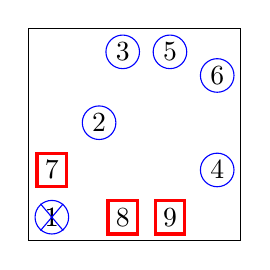
\begin{tikzpicture}[x = 3mm, y=3mm]
	\draw (-1,-1) rectangle (8,8);
	\tikzstyle{Square} = [
		draw = red, 
		very thick,
		rectangle,
		inner sep = 1mm,
		minimum size = 3 mm
	]
	\tikzstyle{SquareFill} = [
		draw = red, 
		fill = red,
		very thick,
		rectangle,
	]
	\tikzstyle{Circle} = [
		draw = blue, 
		circle,
		inner sep = 0.5 mm
	]
	\tikzstyle{CircleFill} = [
		draw = blue,
		fill = blue, 
		circle,
	]
	\node [Circle] (1) at (0,0) {1};
	\node [Circle] (2) at (2,4) {2};
	\node [Circle] (3) at (3,7) {3};
	\node [Circle] (4) at (7,2) {4};
	\node [Circle] (5) at (5,7) {5};
	\node [Circle] (6) at (7,6) {6};
	\node [Square] (7) at (0,2) {7};
	\node [Square] (8) at (3,0) {8};
	\node [Square] (9) at (5,0) {9};

	\node [Circle, cross out] (1) at (0,0) {1};
\end{tikzpicture}
\end{center}



Our original dataset has 619,027 samples.  We first removed the 27,723 crashes involving a pedestrian, leaving 591,304 samples.  Each sample had 82 features; we cut the number of features to 38 for our ``Hard'' features, then to 21 for ``Medium,'' and to 10 for ``Easy.''  We then split each of those three datasets 70/30 into a training set of 413,913 samples and a test set of 177,393 samples, preserving the proportions of negative and positive samples in both sets.  We did the train/test split twice with different random seeds (``Round 1'' and ``Round 2'') to gauge how much of the small differences in results were due to stochasticity instead of differences in the model algorithms or hyperparameters.  Tomek undersampling only applies to the training set, not to the test set.  

We then ran Imbalanced-Learn's  TomekLinks algorithm, then ran it again on the results to give our ``Tomek Once'' and ``Tomek Twice'' undersampled datasets.  

\

\hfil\begin{tabular}{lrrl}
\multicolumn{2}{l}{Hard Features, Round 1}   &  & \cr
 & Samples & \multicolumn{2}{c}{Change} \cr\hline
Original & 413,913 &  & \cr
Tomek Once & 399,515 & 14,398 & 3.48\%\cr
Tomek Twice & 396,511 & 3,004 & 0.75\%\cr\cline{3-4}
Total Change &  & 17,402 & 4.23\%\cr
\end{tabular}
\qquad\begin{tabular}{lrrl}
\multicolumn{2}{l}{Hard Features, Round 2} & \cr
 & Samples & \multicolumn{2}{c}{Change} \cr\hline
Original & 413,913 &  & \cr
Tomek Once & 399,714 & 14,199 & 3.43\%\cr
Tomek Twice & 396,718 & 2,996 & 0.75\%\cr\cline{3-4}
Total Change &  & 17,195 & 4.18\%\cr
\end{tabular}

\vskip 12pt

\hfil\begin{tabular}{lrrl}
\multicolumn{3}{l}{Medium Features, Round 1} & \cr
 & Samples & \multicolumn{2}{c}{Change} \cr\hline
Original & 413,913 &  & \cr
Tomek Once & 406,691 & 7,222 & 1.74\%\cr
Tomek Twice & 405,288 & 1,403 & 0.34\%\cr\cline{3-4}
Total Change &  & 8,625 & 2.08\%\cr
\end{tabular}
\qquad
\begin{tabular}{lrrl}
\multicolumn{3}{l}{Medium Features, Round 2} & \cr
 & Samples & \multicolumn{2}{c}{Change} \cr\hline
Original & 413,913 &  & \cr
Tomek Once & 406,781 & 7,132 & 1.72\%\cr
Tomek Twice & 405,368 & 1,413 & 0.35\%\cr\cline{3-4}
Total Change &  & 8,545 & 2.07\%\cr
\end{tabular}

\vskip 12pt

\hfil\begin{tabular}{lrrl}
\multicolumn{2}{l}{Easy Features, Round 1} & \cr
 & Samples & \multicolumn{2}{c}{Change} \cr\hline
Original & 413,913 &  & \cr
Tomek Once & 413,909 & 4 & 0.00097\%\cr
Tomek Twice & 413,908 & 1 & 0.00024\%\cr\cline{3-4}
Total Change &  & 5 & 0.00121\%\cr
\end{tabular}
\qquad
\begin{tabular}{lrrl}
\multicolumn{2}{l}{Easy Features, Round 2} & \cr
 & Samples & \multicolumn{2}{c}{Change} \cr\hline
Original & 413,913 &  & \cr
Tomek Once & 413,908 & 5 & 0.00121\%\cr
Tomek Twice & 413,907 & 1 & 0.00024\%\cr\cline{3-4}
Total Change &  & 6 & 0.00145\%\cr
\end{tabular}

\

We ran the models on the two rounds of Tomek undersampled training for the Hard-feature and Medium-feature sets, not for the Easy because the undersampling was so small.  

We were disappointed to not see a significant improvement in the model metrics from the undersampling; the difference between no undersampling, one runs of Tomek, and two runs turned out to be inconsequential, by which we mean that one approach was not consistently better when we ran the models with different random seeds.  


\subsubsection{Modifying the Loss Function}

A popular and well established way to modify the loss function for imbalanced data is with class weights, which can have the same effect as na{\"i}ve oversampling.  

Three of our seven models take class weights, and for those we tried three different class weights.  The Tomek undersampling changes the last weight slightly from $0.8499$ to as low as $0.8433$.

\

\hfil\begin{tabular}{c|l}
	$\alpha$ & Meaning \cr\hline
	1/2 & No class weight \cr
	2/3 & $\Delta FP/\Delta TP < 2.0$ goal \cr
	$0.85$ & Balanced classes \cr 
\end{tabular}

\


A related method is with focal loss, which has a modulating hyperparameter $\gamma$ that increases the penalty for low-confidence samples. \citep{lin2017focal}  We tried five values  of $\gamma$.

\

\hfil\begin{tabular}{c|c}
	$\gamma$  & Notes \cr\hline
	0.0 & Same as binary crossentropy \cr
	0.5 & Very light modulation \cr
	1.0 & Light modulation\cr
	2.0 & Recommended by Lin \cr
	5.0 & Heavy modulation \cr
\end{tabular}	

\

We did not see significant improvement using focal loss.  ({\bf Put in Label Reference}).

%%%
\subsubsection{Metrics for Imbalance}

In the \nameref{Methods_Metrics} subsection above we defined the metrics recall, precision, and f1.  The most common metric in machine learning, the one that most algorithms are designed to maximize, is accuracy, the proportion of samples correctly classified.  In that section's example of transformed model output, we had 150,107 out of 177,392 test samples correctly classified, giving 84.6\% accuracy.  Is that good?  The model below, the raw results of the Logistic Regression model of the easy features set, recommends sending no ambulances, and it is correct in 150,771 of 177,392 test samples, giving 84.99\% accuracy.  Is that better?



\

%%%
\parbox{\linewidth}{
%{\bf Balanced Random Forest model, Hard features, No Tomek, $\alpha = 2/3$}

\noindent\begin{tabular}{@{\hspace{-6pt}}p{2.3in} @{\hspace{-6pt}}p{2.0in} p{1.8in}}
	\vskip 0pt
	\qquad \qquad Raw Model Output
	
	\input{../Keras/Images/LRC_Easy_Tomek_0_alpha_0_5_v1_Pred.pgf}
&
	\vskip 0pt
	\qquad \qquad ROC Curve
	
	\input{../Keras/Images/LRC_Easy_Tomek_0_alpha_0_5_v1_ROC.pgf}
	
&
	\vskip 0pt
	\begin{tabular}{cc|c|c|}
	&\multicolumn{1}{c}{}& \multicolumn{2}{c}{Prediction} \cr
	&\multicolumn{1}{c}{} & \multicolumn{1}{c}{N} & \multicolumn{1}{c}{P} \cr\cline{3-4}
	\multirow{2}{*}{\rotatebox[origin=c]{90}{Actual}}&N &
150,771 & 0
	\vrule width 0pt height 10pt depth 2pt \cr\cline{3-4}
	&P & 
26621 & 0
	\vrule width 0pt height 10pt depth 2pt \cr\cline{3-4}
	\end{tabular}

	\hfil\begin{tabular}{ll}
	\cr
	0.8499 & Accuracy\cr
und & Precision \cr	0.0 & Recall \cr	und & F1 \cr	0.659 & AUC \cr
\end{tabular}

\cr
\end{tabular}
} % End parbox

\

In this study, we  have arbitrarily decided that we are willing to trade off up to two false positives to get one more true positive.  Once we moved our decision thresholds to the ethical tradeoff point, the accuracy only varied from 0.836 to 0.854.  The difference in accuracy tells us how many more (or fewer) false positives than true positives we have, with them being equal at 0.8499, and we get the same information from precision being less than, more than, or equal to 0.5.    Therefore, we are not going to consider accuracy in evaluating our models. 

%%%
\subsubsection{ML Algorithms for Imbalanced Data}

{\bf [Expand this subsubsection]}

\begin{itemize}
	\item Random Undersampling Composite Models
	\item Bagging
	\item Boosting
\end{itemize}

%%%%%
\subsection{Models}

We used seven binary classification algorithms.  Three of them take class weights.

\

\hfil\begin{tabular}{llc}
&& Class \cr
Model & Source & Weights \cr\hline
KerasClassifier with the Binary Focal Crossentropy loss function & Keras & Yes \cr
Balanced Random Forest Classifier & Imbalanced-Learn & Yes \cr
Balanced Bagging Classifier & Imbalanced-Learn & No \cr
RUSBoost Classifier & Imbalanced-Learn & No \cr
Easy Ensemble Classifier with AdaBoost Estimator & Imbalanced-Learn & No \cr
Logistic Regression Classifier & Scikit-Learn & Yes \cr
AdaBoost  Classifier & Scikit-Learn & No \cr
\end{tabular}

\


For the focal loss function, we tried seven different combinations of the hyperparameters $\alpha$ for class weights and $\gamma$ for penalty on badly misclassified samples.  For the random forest and bagging models we tried three values of $\alpha$.  Altogether we had seventeen model/hyperparameter combinations.  We learned each of the seven models on datasets with the easy, medium, and hard features, and on the hard features we tested with Tomek undersampling 0, 1, and 2 times, for a total of five datasets, giving eighty-five model/hyperparameter/dataset combinations.    We learned each of those sixty-five with two different random seeds, for a total of one hundred seventy results.  

\

\hfil\noindent\begin{tabular}{ccc}
	\multicolumn{3}{c}{Seventeen Models} \cr
	Model & $\alpha$ & $\gamma$ \cr\hline
	Focal & 1/2 & 0.0 \cr
	Focal & 2/3 & 0.0 \cr
	Focal & 2/3 & 0.5 \cr
	Focal & 2/3 & 1.0 \cr
	Focal & 2/3 & 2.0 \cr
	Focal & 2/3 & 5.0 \cr
	Focal & 0.85 & 0.0 \cr
	Random Forest & 1/2 & \cr
	Random Forest & 2/3 & \cr
	Random Forest & 0.85 & \cr
	Bagging && \cr
	RUSBoost && \cr
	Easy Ens && \cr
	Log Reg & 1/2 & \cr
	Log Reg & 2/3 & \cr
	Log Reg & 0.85 & \cr
	AdaBoost && \cr
\end{tabular}
\quad
$\times$
\quad
\begin{tabular}{cc}
	\multicolumn{2}{c}{Seven Datasets} \cr
	Features & Tomek \cr\hline
	Hard & None \cr
	Hard & Once \cr
	Hard & Twice \cr
	Medium & None \cr
	Medium & Once \cr
	Medium & Twice \cr
	Easy & None \cr
\end{tabular}
\quad
$\times$
\quad
\begin{tabular}{cc}
	Run twice with \cr
	different \cr
	random seeds \cr\hline
	Random seed 1 \cr
	Random seed 2
\end{tabular}
\quad 
$=$ 
\quad 
\begin{tabular}{c}
	238  \cr Sets of  \cr
	Results \cr
\end{tabular}









%%%%% Results
\section{Results}\label{Results}
%%%%%
% Headline Results
\subsection{More Features Improve the Model}

Our model metrics show that having more information about each crash and crash person greatly increases the precision and recall of the model.  The graphs and metrics below show the model with the highest F1 score for each of the easy, medium, and hard sets of features.  In terms of F1, all of the easy-feature models were worse than all of the medium-feature models, and except for the Easy Ensemble Classifier models, all of the medium-feature models were worse than the hard-feature models.  
Full details about features for each set is in \verb|CRSS_06_Build_Model_01_15_22.ipynb|.


The Easy set of features assumes that the automated crash notification comes to the police only with a location and that the police do not correlate that location information with detailed maps for information like whether that location is in a parking lot or a high-speed intersection.  These features (day of week, time of day, weather,...) are information the police already had before the notification.  This model balanced bagging model does correctly tell the police to dispatch 1,656 ambulances immediately with 40.0\% precision, which is better than zero.  



\

%%%
\parbox{\linewidth}{
{\bf Easy Features:  Balanced Random Forest model, No Tomek undersampling, No class weights}

\noindent\begin{tabular}{@{\hspace{-6pt}}p{2.3in} @{\hspace{-6pt}}p{2.0in} p{1.8in}}
	\vskip 0pt
	\hfil Raw Model Output
	
	\input{../Keras/Images/BRFC_Easy_Tomek_0_alpha_0_5_v2_Pred.pgf}
	
&
	\vskip 0pt
	\hfil Linear Transformation
	
	\input{../Keras/Images/BRFC_Easy_Tomek_0_alpha_0_5_v2_Linear_Transform_Pred.pgf}

&
	\vskip 0pt
	\begin{tabular}{cc|c|c|}
	&\multicolumn{1}{c}{}& \multicolumn{2}{c}{Prediction} \cr
	&\multicolumn{1}{c}{} & \multicolumn{1}{c}{N} & \multicolumn{1}{c}{P} \cr\cline{3-4}
	\multirow{2}{*}{\rotatebox[origin=c]{90}{Actual}}&N &
148,287 & 2,484
	\vrule width 0pt height 10pt depth 2pt \cr\cline{3-4}
	&P & 
24,965 & 1,656
	\vrule width 0pt height 10pt depth 2pt \cr\cline{3-4}
	\end{tabular}

	\hfil\begin{tabular}{ll}
	\cr
0.400 & Precision \cr	0.062 & Recall \cr	0.108 & F1 \cr	0.664 & AUC \cr	0.857 & $p$ \cr
	\end{tabular}

\cr
\end{tabular}
} % End parbox

The Medium features assume two things.

\begin{enumerate}
	\item The police can correlate the location with detailed maps to get, for instance, the kind of road and whether the crash was in an intersection
	\item The automated cell phone crash report comes to the police from the cell service provider with some information about the likely user of the phone, including age and sex.  
\end{enumerate}
	
	Our best model on the Medium features sends $6,464$ needed ambulances with $43.0\%$ precision, much better than the Easy features.  Using this improved recall and precision is a good argument for investing in the data infrastructure necessary to make this information instantaneously available.  

\

%%%
\parbox{\linewidth}{
{\bf Medium Features:  Balanced Radom Forest model, Tomek Once, No class weights}

\noindent\begin{tabular}{@{\hspace{-6pt}}p{2.3in} @{\hspace{-6pt}}p{2.0in} p{1.8in}}
	\vskip 0pt
	\qquad \qquad Raw Model Output
	
	\input{../Keras/Images/BRFC_Medium_Tomek_1_alpha_0_5_v2_Pred.pgf}
	
&
	\vskip 0pt
	\qquad \qquad Linear Transformation
	
	\input{../Keras/Images/BRFC_Medium_Tomek_1_alpha_0_5_v2_Linear_Transform_Pred.pgf}

&
	\vskip 0pt
	\begin{tabular}{cc|c|c|}
	&\multicolumn{1}{c}{}& \multicolumn{2}{c}{Prediction} \cr
	&\multicolumn{1}{c}{} & \multicolumn{1}{c}{N} & \multicolumn{1}{c}{P} \cr\cline{3-4}
	\multirow{2}{*}{\rotatebox[origin=c]{90}{Actual}}&N &
142,217 & 8,554
	\vrule width 0pt height 10pt depth 2pt \cr\cline{3-4}
	&P & 
20,157 & 6,464
	\vrule width 0pt height 10pt depth 2pt \cr\cline{3-4}
	\end{tabular}

	\hfil\begin{tabular}{ll}
	\cr
0.430 & Precision \cr	0.243 & Recall \cr	0.310 & F1 \cr	0.728 & AUC \cr	0.763 & $p$ \cr
	\end{tabular}
\cr
\end{tabular}
} % End parbox

The Hard features assume that the police can do an additional three things.  

\begin{enumerate}
	\item Correlate information about the likely phone user with public and private records about automobile ownership and insurance to guess what kind of vehicle the person is driving
	\item Correlate location with detailed and up-to-date maps of lighting conditions and work zones.  
	\item Correlate multiple notifications from the same location to determine (minimum) number of passengers, including whether a school bus is involved.  
\end{enumerate}

	Our best model on the Hard features sends $10,397$ needed ambulances with $51.3\%$ precision.  Again, this improvement in both precision and recall are good arguments for investing in the needed additional data infrastructure.

\

%%%
\parbox{\linewidth}{
{\bf Hard Features:  Balanced Random Forest model, Tomek twice, No class weights}

\noindent\begin{tabular}{@{\hspace{-6pt}}p{2.3in} @{\hspace{-6pt}}p{2.0in} p{1.8in}}
	\vskip 0pt
	\qquad \qquad Raw Model Output
	
	\input{../Keras/Images/BRFC_Hard_Tomek_2_alpha_0_5_v1_Pred.pgf}
	
&
	\vskip 0pt
	\qquad \qquad Linear Transformation
	
	\input{../Keras/Images/BRFC_Hard_Tomek_2_alpha_0_5_v1_Linear_Transform_Pred.pgf}

&
	\vskip 0pt
	\begin{tabular}{cc|c|c|}
	&\multicolumn{1}{c}{}& \multicolumn{2}{c}{Prediction} \cr
	&\multicolumn{1}{c}{} & \multicolumn{1}{c}{N} & \multicolumn{1}{c}{P} \cr\cline{3-4}
	\multirow{2}{*}{\rotatebox[origin=c]{90}{Actual}}&N &
140,914 & 9,857
	\vrule width 0pt height 10pt depth 2pt \cr\cline{3-4}
	&P & 
16,224 & 10,397
	\vrule width 0pt height 10pt depth 2pt \cr\cline{3-4}
	\end{tabular}

	\hfil\begin{tabular}{ll}
	\cr
0.513 & Precision \cr	0.391 & Recall \cr	0.444 & F1 \cr	0.800 & AUC \cr	0.705 & $p$ \cr
	\end{tabular}

\cr
\end{tabular}
} % End parbox


\subsection{Results of Undersampling and Hyperparameters}

The table below shows the top thirty-two runs measured by the F1 score, and the top run for each of the five remaining model algorithms.  All of the results are for the hard features.  

The second column tells how many times we ran Tomek undersampling.  The third column gives the values of the hyperparameters $\alpha$ (class weight) that we used for the Balanced Random Forest, Keras Binary Focal Loss classifier, and Logistic Regression classifiers.  The fourth column gives the values of $\gamma$ (focal weight) we varied for the Keras binary focal loss classifier.  We ran the models twice with different random seeds (``Round 1'' and ``Round 2'' below), to see whether small differences were due to different models and hyperparameters or due to the inherent stochasticity of the train/test split and machine learning algorithms.  

\

\hfil\begin{tabular}{*9{c}}
Algorithm & Tomek & $\alpha$ & $\gamma$ & Round & Precision & Recall & F1 & AUC \cr\hline
BRFC & 2 & 1/2 && 1 & 0.5133 & 0.3906 & 0.4436 & 0.8002 \cr
BRFC & 1 & 1/2 && 1 & 0.5136 & 0.3880 & 0.4420 & 0.7998 \cr
BRFC & 0 & 1/2 && 1 & 0.5145 & 0.3858 & 0.4410 & 0.7993 \cr
BRFC & 2 & 2/3 && 1 & 0.5064 & 0.3904 & 0.4409 & 0.7997 \cr
BRFC & 0 & 2/3 && 1 & 0.5107 & 0.3866 & 0.4401 & 0.7995 \cr
BRFC & 0 & 0.85 && 1 & 0.5056 & 0.3892 & 0.4399 & 0.7986 \cr
BRFC & 1 & 2/3 && 1 & 0.5093 & 0.3866 & 0.4396 & 0.7994 \cr
BRFC & 2 & 1/2 && 2 & 0.5061 & 0.3857 & 0.4378 & 0.7982 \cr
BRFC & 2 & 0.85 && 1 & 0.5054 & 0.3823 & 0.4353 & 0.7984 \cr
BRFC & 1 & 1/2 && 2 & 0.5069 & 0.3810 & 0.4350 & 0.7977 \cr
BRFC & 1 & 2/3 && 2 & 0.5041 & 0.3824 & 0.4349 & 0.7981 \cr
BRFC & 1 & 0.85 && 2 & 0.5036 & 0.3801 & 0.4332 & 0.7967 \cr
BRFC & 1 & 0.85 && 1 & 0.5185 & 0.3673 & 0.4300 & 0.7978 \cr
BRFC & 2 & 0.85 && 2 & 0.5078 & 0.3702 & 0.4282 & 0.7970 \cr
BRFC & 0 & 1/2 && 2 & 0.5173 & 0.3649 & 0.4280 & 0.7967 \cr
BRFC & 0 & 2/3 && 2 & 0.5166 & 0.3652 & 0.4279 & 0.7977 \cr
BRFC & 2 & 2/3 && 2 & 0.5123 & 0.3667 & 0.4274 & 0.7973 \cr
BRFC & 0 & 0.85 && 2 & 0.5091 & 0.3652 & 0.4253 & 0.7961 \cr\hline
KBFC & 1 & 1/2  & 0.0 & 1 & 0.4825 & 0.3270 & 0.3898 & 0.7758 \cr
KBFC & 0 & 1/2  & 0.0 & 1 & 0.4850 & 0.3196 & 0.3853 & 0.7753 \cr
KBFC & 1 & 2/3  & 0.0 & 1 & 0.4848 & 0.3164 & 0.3829 & 0.7758 \cr
KBFC & 0 & 2/3  & 0.5 & 2 & 0.4757 & 0.3202 & 0.3828 & 0.7755 \cr
KBFC & 0 & 2/3  & 0.0 & 2 & 0.4790 & 0.3187 & 0.3827 & 0.7750 \cr
Bagging & 2 &&& 1 & 0.5043 & 0.3079 & 0.3823 & 0.7664 \cr
KBFC & 0 & 2/3  & 1.0 & 2 & 0.4805 & 0.3166 & 0.3817 & 0.7748 \cr
KBFC & 1 & 0.85  & 0.0 & 1 & 0.4722 & 0.3199 & 0.3815 & 0.7742 \cr
KBFC & 2 & 2/3  & 0.0 & 1 & 0.4830 & 0.3152 & 0.3814 & 0.7744 \cr
KBFC & 2 & 2/3  & 0.5 & 1 & 0.4912 & 0.3117 & 0.3814 & 0.7751 \cr
KBFC & 2 & 1/2  & 0.0 & 1 & 0.4886 & 0.3125 & 0.3812 & 0.7743 \cr
KBFC & 2 & 2/3  & 1.0 & 1 & 0.4874 & 0.3127 & 0.3810 & 0.7750 \cr
KBFC & 1 & 2/3  & 1.0 & 1 & 0.4855 & 0.3131 & 0.3807 & 0.7751 \cr
KBFC & 1 & 2/3  & 0.5 & 2 & 0.4747 & 0.3171 & 0.3802 & 0.7740 \cr\vdots \cr
LRC & 1 & 1/2 && 1 & 0.4408 & 0.2895 & 0.3495 & 0.7548 \cr
AdaBoost & 2 &&& 1 & 0.4408 & 0.2707 & 0.3354 & 0.7542 \cr
RUSBoost & 0 &&& 1 & 0.4412 & 0.2660 & 0.3319 & 0.7547 \cr
EEC & 0 &&& 1 & 0.4202 & 0.2488 & 0.3125 & 0.7329 \cr\end{tabular}

\

The results indicate that Tomek undersampling and focal loss do not make a significant difference, especially compared with the much larger difference between the worst Balanced Random Forest Classifier model and the best Keras Binary Focal Crossentropy model.  Though varying the hyperparameters did not give the most significant changes in the results, we found interesting behaviors that may be relevant to future research.  What makes our look at focal loss different from most study is that we are only interested in the right tail past where $\Delta FP/\Delta TP = 2.0$.  




%%%%%
\subsection{Varying Binary Focal Crossentropy Hyperparameters}

The Binary Focal Crossentropy loss function for Keras's neural network algorithm takes both a class weight hyperparameter $\alpha$ and a modulating factor hyperparameter $\gamma$ that gives more weight to samples badly misclassified.  We tried combinations, including the values of $\gamma$ tested in the paper \cite{lin2017focal}  The balanced class weight will vary slightly with undersampling of the majority class.  

\

\hfil\begin{tabular}{c|c}
	$\alpha$ & Meaning \cr\hline
	1/2 & No class weight  \cr
	2/3 & $\Delta FP/\Delta TP < 2$  \cr
	0.85 & Balanced class weight  \cr
	\multicolumn{2}{c}{}\cr
	\multicolumn{2}{c}{}\cr
\end{tabular}	
\qquad\begin{tabular}{c|c}
	$\gamma$  & Notes \cr\hline
	0.0 & Same as binary crossentropy \cr
	0.5 & Very light modulation \cr
	1.0 & Light modulation\cr
	2.0 & Recommended by Lin \cr
	5.0 & Heavy modulation \cr
\end{tabular}	

\subsubsection{Varying Class Weights}

All three models used no Tomek undersampling and $\gamma=0.0$.

With $\alpha = 0.5$, the model classifies the negative class well, but the positive class almost randomly.  With $\alpha = 0.85$, balanced class weights, the model classifies the positive class well, but the positive class so poorly that the model does not separate the two classes well.  

\

%%%
\parbox{\linewidth}{
{ No class weight ($\alpha = 0.5$)}

\noindent\begin{tabular}{@{\hspace{-6pt}}p{2.3in} @{\hspace{-6pt}}p{2.0in} p{1.8in}}
	\vskip 0pt
	\hfil Raw Model Output
	
	\input{../Keras/Images/KBFC_Hard_Tomek_0_alpha_0_5_gamma_0_0_v1_Pred.pgf}
	
&
	\vskip 0pt
	\hfil Linear Transformation
	
	\input{../Keras/Images/KBFC_Hard_Tomek_0_alpha_0_5_gamma_0_0_v1_Linear_Transform_Pred.pgf}

&
	\vskip 0pt
	\begin{tabular}{cc|c|c|}
	&\multicolumn{1}{c}{}& \multicolumn{2}{c}{Prediction} \cr
	&\multicolumn{1}{c}{} & \multicolumn{1}{c}{N} & \multicolumn{1}{c}{P} \cr\cline{3-4}
	\multirow{2}{*}{\rotatebox[origin=c]{90}{Actual}}&N &
141736 & 9035
	\vrule width 0pt height 10pt depth 2pt \cr\cline{3-4}
	&P & 
18113 & 8508
	\vrule width 0pt height 10pt depth 2pt \cr\cline{3-4}
	\end{tabular}

	\hfil\begin{tabular}{ll}
	\cr
	0.485 & Precision \cr	0.320 & Recall \cr	0.385 & F1 \cr	0.775 & AUC \cr 0.546 & $p$ \cr
	\end{tabular}

\cr
\end{tabular}
} % End parbox

%%%
\parbox{\linewidth}{
{ Class weight for $\Delta FP/\Delta TP=2.0$ ($\alpha = 2/3$)}

\noindent\begin{tabular}{@{\hspace{-6pt}}p{2.3in} @{\hspace{-6pt}}p{2.0in} p{1.8in}}
	\vskip 0pt
	\hfil Raw Model Output
	
	\input{../Keras/Images/KBFC_Hard_Tomek_0_alpha_target_gamma_0_0_v1_Pred.pgf}
	
&
	\vskip 0pt
	\hfil Linear Transformation
	
	\input{../Keras/Images/KBFC_Hard_Tomek_0_alpha_target_gamma_0_0_v1_Linear_Transform_Pred.pgf}

&
	\vskip 0pt
	\begin{tabular}{cc|c|c|}
	&\multicolumn{1}{c}{}& \multicolumn{2}{c}{Prediction} \cr
	&\multicolumn{1}{c}{} & \multicolumn{1}{c}{N} & \multicolumn{1}{c}{P} \cr\cline{3-4}
	\multirow{2}{*}{\rotatebox[origin=c]{90}{Actual}}&N &
142029 & 8742	
	\vrule width 0pt height 10pt depth 2pt \cr\cline{3-4}
	&P & 
18346 & 8275
	\vrule width 0pt height 10pt depth 2pt \cr\cline{3-4}
	\end{tabular}

	\hfil\begin{tabular}{ll}
	\cr
	0.486 & Precision \cr	0.311 & Recall \cr	0.379 & F1 \cr	0.774 & AUC \cr 0.711 & $p$ \cr
	\end{tabular}

\cr
\end{tabular}
} % End parbox

%%%

\parbox{\linewidth}{

{ Class weight for class balance ($\alpha \approx 0.85$)}

\noindent\begin{tabular}{@{\hspace{-6pt}}p{2.3in} @{\hspace{-6pt}}p{2.0in} p{1.8in}}
	\vskip 0pt
	\hfil Raw Model Output
	
	\input{../Keras/Images/KBFC_Hard_Tomek_0_alpha_balanced_gamma_0_0_v1_Pred.pgf}
	
&
	\vskip 0pt
	\hfil Linear Transformation
	
	\input{../Keras/Images/KBFC_Hard_Tomek_0_alpha_balanced_gamma_0_0_v1_Linear_Transform_Pred.pgf}

&
	\vskip 0pt
	\begin{tabular}{cc|c|c|}
	&\multicolumn{1}{c}{}& \multicolumn{2}{c}{Prediction} \cr
	&\multicolumn{1}{c}{} & \multicolumn{1}{c}{N} & \multicolumn{1}{c}{P} \cr\cline{3-4}
	\multirow{2}{*}{\rotatebox[origin=c]{90}{Actual}}&N &
141975 & 8796
	\vrule width 0pt height 10pt depth 2pt \cr\cline{3-4}
	&P & 
18339 & 8282
	\vrule width 0pt height 10pt depth 2pt \cr\cline{3-4}
	\end{tabular}

	\hfil\begin{tabular}{ll}
	\cr
0.485 & Precision \cr	0.311 & Recall \cr	0.379 & F1 \cr	0.774 & AUC \cr 0.892 & $p$ \cr
	\end{tabular}

\cr
\end{tabular}
} % End parbox

\

%%%%%
\subsubsection{Varying $\gamma$ for Focal Loss}

All five models used the class weight for $\Delta FP/\Delta TP=2.0$, $\alpha = 2/3$, with no Tomek undersampling.  

The aspect that caught our attention was the way larger focal weights make the probabilities clusters towards the center, rather than the desired effect of giving more strongly classified samples.  

\

%%%
\parbox{\linewidth}{
{ $\gamma = 0.0$, same as non-focal binary crossentropy}

\noindent\begin{tabular}{@{\hspace{-6pt}}p{2.3in} @{\hspace{-6pt}}p{2.0in} p{1.8in}}
	\vskip 0pt
	\hfil Raw Model Output
	
	\input{../Keras/Images/KBFC_Hard_Tomek_0_alpha_target_gamma_0_0_v1_Pred.pgf}
	
&
	\vskip 0pt
	\hfil Linear Transformation
	
	\input{../Keras/Images/KBFC_Hard_Tomek_0_alpha_target_gamma_0_0_v1_Linear_Transform_Pred.pgf}

&
	\vskip 0pt
	\begin{tabular}{cc|c|c|}
	&\multicolumn{1}{c}{}& \multicolumn{2}{c}{Prediction} \cr
	&\multicolumn{1}{c}{} & \multicolumn{1}{c}{N} & \multicolumn{1}{c}{P} \cr\cline{3-4}
	\multirow{2}{*}{\rotatebox[origin=c]{90}{Actual}}&N &
142029 & 8742	
	\vrule width 0pt height 10pt depth 2pt \cr\cline{3-4}
	&P & 
18346 & 8275
	\vrule width 0pt height 10pt depth 2pt \cr\cline{3-4}
	\end{tabular}

	\hfil\begin{tabular}{ll}
	\cr
	0.486 & Precision \cr	0.311 & Recall \cr	0.379 & F1 \cr	0.774 & AUC \cr 0.711 & $p$ \cr
	\end{tabular}

\cr
\end{tabular}
} % End parbox

%%%
\parbox{\linewidth}{
{ $\gamma = 0.5$}

\noindent\begin{tabular}{@{\hspace{-6pt}}p{2.3in} @{\hspace{-6pt}}p{2.0in} p{1.8in}}
	\vskip 0pt
	\hfil Raw Model Output
	
	\input{../Keras/Images/KBFC_Hard_Tomek_0_alpha_target_gamma_0_5_v1_Pred.pgf}
	
&
	\vskip 0pt
	\hfil Linear Transformation
	
	\input{../Keras/Images/KBFC_Hard_Tomek_0_alpha_target_gamma_0_5_v1_Linear_Transform_Pred.pgf}

&
	\vskip 0pt
	\begin{tabular}{cc|c|c|}
	&\multicolumn{1}{c}{}& \multicolumn{2}{c}{Prediction} \cr
	&\multicolumn{1}{c}{} & \multicolumn{1}{c}{N} & \multicolumn{1}{c}{P} \cr\cline{3-4}
	\multirow{2}{*}{\rotatebox[origin=c]{90}{Actual}}&N &
142202 & 8569
	\vrule width 0pt height 10pt depth 2pt \cr\cline{3-4}
	&P & 
18492 & 8129
	\vrule width 0pt height 10pt depth 2pt \cr\cline{3-4}
	\end{tabular}

	\hfil\begin{tabular}{ll}
	\cr
0.487 & Precision \cr	0.305 & Recall \cr	0.375 & F1 \cr	0.774 & AUC \cr	0.655 & $p$ \cr
	\end{tabular}

\cr
\end{tabular}
} % End parbox


%%%
\parbox{\linewidth}{
{ $\gamma = 1.0$}

\noindent\begin{tabular}{@{\hspace{-6pt}}p{2.3in} @{\hspace{-6pt}}p{2.0in} p{1.8in}}
	\vskip 0pt
	\hfil Raw Model Output
	
	\input{../Keras/Images/KBFC_Hard_Tomek_0_alpha_target_gamma_1_0_v1_Pred.pgf}
	
&
	\vskip 0pt
	\hfil Linear Transformation
	
	\input{../Keras/Images/KBFC_Hard_Tomek_0_alpha_target_gamma_1_0_v1_Linear_Transform_Pred.pgf}

&
	\vskip 0pt
	\begin{tabular}{cc|c|c|}
	&\multicolumn{1}{c}{}& \multicolumn{2}{c}{Prediction} \cr
	&\multicolumn{1}{c}{} & \multicolumn{1}{c}{N} & \multicolumn{1}{c}{P} \cr\cline{3-4}
	\multirow{2}{*}{\rotatebox[origin=c]{90}{Actual}}&N &
141630 & 9141
	\vrule width 0pt height 10pt depth 2pt \cr\cline{3-4}
	&P & 
18242 & 8379
	\vrule width 0pt height 10pt depth 2pt \cr\cline{3-4}
	\end{tabular}

	\hfil\begin{tabular}{ll}
	\cr
0.478 & Precision \cr	0.315 & Recall \cr	0.380 & F1 \cr	0.775 & AUC \cr	0.615 & $p$ \cr
	\end{tabular}

\cr
\end{tabular}
} % End parbox


%%%
\parbox{\linewidth}{
{ $\gamma = 2.0$}

\noindent\begin{tabular}{@{\hspace{-6pt}}p{2.3in} @{\hspace{-6pt}}p{2.0in} p{1.8in}}
	\vskip 0pt
	\hfil Raw Model Output
	
	\input{../Keras/Images/KBFC_Hard_Tomek_0_alpha_target_gamma_2_0_v1_Pred.pgf}
	
&
	\vskip 0pt
	\hfil Linear Transformation
	
	\input{../Keras/Images/KBFC_Hard_Tomek_0_alpha_target_gamma_2_0_v1_Linear_Transform_Pred.pgf}

&
	\vskip 0pt
	\begin{tabular}{cc|c|c|}
	&\multicolumn{1}{c}{}& \multicolumn{2}{c}{Prediction} \cr
	&\multicolumn{1}{c}{} & \multicolumn{1}{c}{N} & \multicolumn{1}{c}{P} \cr\cline{3-4}
	\multirow{2}{*}{\rotatebox[origin=c]{90}{Actual}}&N &
142496 & 8275
	\vrule width 0pt height 10pt depth 2pt \cr\cline{3-4}
	&P & 
18602 & 8019
	\vrule width 0pt height 10pt depth 2pt \cr\cline{3-4}
	\end{tabular}

	\hfil\begin{tabular}{ll}
	\cr
0.492 & Precision \cr	0.301 & Recall \cr	0.374 & F1 \cr	0.774 & AUC \cr	0.585 & $p$ \cr
	\end{tabular}

\cr
\end{tabular}
} % End parbox


%%%
\parbox{\linewidth}{
{ $\gamma = 5.0$}

\noindent\begin{tabular}{@{\hspace{-6pt}}p{2.3in} @{\hspace{-6pt}}p{2.0in} p{1.8in}}
	\vskip 0pt
	\hfil Raw Model Output
	
	\input{../Keras/Images/KBFC_Hard_Tomek_0_alpha_target_gamma_5_0_v1_Pred.pgf}
	
&
	\vskip 0pt
	\hfil Linear Transformation
	
	\input{../Keras/Images/KBFC_Hard_Tomek_0_alpha_target_gamma_5_0_v1_Linear_Transform_Pred.pgf}

&
	\vskip 0pt
	\begin{tabular}{cc|c|c|}
	&\multicolumn{1}{c}{}& \multicolumn{2}{c}{Prediction} \cr
	&\multicolumn{1}{c}{} & \multicolumn{1}{c}{N} & \multicolumn{1}{c}{P} \cr\cline{3-4}
	\multirow{2}{*}{\rotatebox[origin=c]{90}{Actual}}&N &
143657 & 7114
	\vrule width 0pt height 10pt depth 2pt \cr\cline{3-4}
	&P & 
19351 & 7270
	\vrule width 0pt height 10pt depth 2pt \cr\cline{3-4}
	\end{tabular}

	\hfil\begin{tabular}{ll}
	\cr
0.505 & Precision \cr	0.273 & Recall \cr	0.355 & F1 \cr	0.773 & AUC \cr	0.543 & $p$ \cr
	\end{tabular}

\cr
\end{tabular}
} % End parbox


%%%%% Conclusions
\section{Conclusions}\label{Conclusions}

%%%%%
\section{Discussion}\label{Discussion}

%%%%% Future Work
\section{Future Work}\label{FutureWork}

%%%%% Notes
\section{To Do, Notes to Self}
%%%%% Notes
\citep{MA2023103983} uses AdaCost, and uses smartphones to collect vehicle kinematic data in field tests.  It's the only article in TRpC that uses AdaCost.  

%%%%%
\section*{Funding Statement}

%%%%% Conflict of Interest
\section*{Conflict of Interest}

The authors have no relevant financial or non-financial interests to disclose.

%%%%% Acknowledgements
\section*{Acknowledgements}

%George Broussard 
[STUDENT]
contributed to this work in the 
[FUNDED PROGRAM]
%NSF Research Experiences for Undergraduates program.

%%%%% Data Availability
\section*{Data Availability}

The CRSS data is publicly available at 

\url{https://www.nhtsa.gov/crash-data-systems/crash-report-sampling-system}


\begin{comment}
% Figure
\begin{figure}[<options>]
	\centering
		\includegraphics[<options>]{}
	  \caption{}\label{fig1}
\end{figure}


\begin{table}[<options>]
\caption{}\label{tbl1}
\begin{tabular*}{\tblwidth}{@{}LL@{}}
\toprule
  &  \\ % Table header row
\midrule
 & \\
 & \\
 & \\
 & \\
\bottomrule
\end{tabular*}
\end{table}
\end{comment}

% Uncomment and use as the case may be
%\begin{theorem} 
%\end{theorem}

% Uncomment and use as the case may be
%\begin{lemma} 
%\end{lemma}

%% The Appendices part is started with the command \appendix;
%% appendix sections are then done as normal sections
%% \appendix

\section{}\label{}

% To print the credit authorship contribution details
\printcredits

%% Loading bibliography style file
%\bibliographystyle{model1-num-names}
\bibliographystyle{cas-model2-names}

% Loading bibliography database
\bibliography{Paper_Summer_2022.bib}


\begin{comment}
% Biography
\bio{}
% Here goes the biography details.
\endbio

\bio{pic1}
% Here goes the biography details.
\endbio
\end{comment}

\end{document}

